\documentclass[Bachelor, ngerman, UKenglish,biblatex=false]{scrbook}
%------------------------------------------------------------------------------
% This file contains a skeleton thesis for
% a Physics or Astronomy Institute in the University of Bonn

% Specify the thesis type as an option: PhD, Master, Diplom, Bachelor
% Specify the thesis stage as an option: Draft (default), Submit, Final, PILibrary

% Specify the language(s) in the class and then use babel.
% If you need more than one language, give the default language last,
% e.g. ngerman, UKenglish for a thesis in British (UK) English where you want
% to be able to set the language to German for some part of it.

%------------------------------------------------------------------------------
% Pass TeX Live version to the package
% Use command pdflatex --version to find out which version you are running
% Add option backref=false when your thesis is ready to turn off back-referencing
%friedrich 
%\usepackage[backend=bibtex, hyperref=true, style=numeric-comp, sorting=none, block=ragged, firstinits=true]{biblatex}
\usepackage[backend=bibtex8,sorting=none]{biblatex}
% in your bibliography
\usepackage[texlive=2016]{ubonn-thesis}
% Adjustments to standard biblatex style
\usepackage{ubonn-biblatex}

% Glossary package
% \usepackage[acronym,toc,nosuper]{glossaries}
% TikZ packages and libraries
% \usepackage{tikz}
% \usepackage{tikz-3dplot}
% \usepackage{pgfplots}
% \usetikzlibrary{positioning,shapes,arrows}
% \usetikzlibrary{decorations.pathmorphing}
% \usetikzlibrary{decorations.markings}
\usepackage{thesis_defs}

%------------------------------------------------------------------------------
% Instead of colouring  links, cites, table of contents etc.
% put them in a coloured box for the screen version.
% This is probably a good idea when you print your thesis.
% \hypersetup{colorlinks=false,
%   linkbordercolor=blue,citebordercolor=magenta,urlbordercolor=darkgreen
% }

%------------------------------------------------------------------------------
% When writing your thesis it is often helpful to have the date and
% time in the output file. Comment this out for the final version.
%\ifoot[\today{} \thistime]{\today{} \thistime}

% In order to check if your labels are referenced try the refcheck package
% \usepackage{refcheck}

%------------------------------------------------------------------------------
% biblatex is included by ubonn-thesis. Look there for the settings used.
% See the options for settings that can be changed easily.
% For further changes copy the \RequirePackage[...]{biblatex} here
% and include ubonn-thesis with the option biblatex=false.

% Specify the bibliography files here and not at the end!
% Use standard_refs-bibtex if you use bibtex or bibtex8
% and standard_refs-biber  if you use biber
\addbibresource{bib/thesis_refs.bib}
%\addbibresource{bib/standard_refs-bibtex.bib}

\usepackage{physics}
\usepackage{todonotes}
\usepackage{booktabs}

%------------------------------------------------------------------------------
% The following definitions are used to produce the title pages
% needed at various stages
\newcommand{\thesistitle}{Hawking Radiation as Seen by Observers}
\newcommand*{\thesisauthor}{Friedrich Hübner}
\newcommand*{\thesistown}{Jena}
\renewcommand*{\InstituteName}{\PI}
\renewcommand*{\inInstitute}{\inPI}
\renewcommand*{\InstituteAddress}{\PIaddress}
% Adjust \thesisreferee...text depending on male/female referee
\newcommand*{\thesisrefereeonetext}{1.\ Gutachter}
\newcommand*{\thesisrefereeone}{Dr.\ Stefan Förste}
\newcommand*{\thesisrefereetwotext}{2.\ Gutachter}
\newcommand*{\thesisrefereetwo}{Prof.\ Dr.\ Albrecht Klemm}
% Date when thesis was submitted (Master/Diplom)
% Year or Month, Year when thesis was submitted (PhD)
\newcommand*{\thesissubmit}{XX.YY.2018}
% \newcommand*{\thesissubmit}{Month 2018}
% Date of thesis examination (PhD)
\newcommand*{\thesispromotion}{XX.YY.2018}
% Month and year of the final printed version of the thesis
\newcommand*{\thesismonth}{Juli}
\newcommand*{\thesisyear}{2018}
\newcommand*{\thesisnumber}{BONN-IR-2018-XXX}

%------------------------------------------------------------------------------
% The abstract is only needed for the printed version and should be in
% English regardless of the language of the thesis
\newcommand{\thesisabstract}{%
  \begin{otherlanguage}{UKenglish}
    This is your thesis abstract. It may be in a language that is
    different from the rest of your thesis.
  \end{otherlanguage}
}

%------------------------------------------------------------------------------
% \includeonly can be used to select which chapters you want to process
% A simple \include command just inserts a \clearpage before and after the file
% Note that \includeonly can be quite picky! Do not forget to put a
% comma after the filename, otherwise it will simply be ignored!
% \includeonly{%
%   thesis_intro,
%   thesis_appendix,
%   thesis_acknowledge,
%	chapter/qft,
%	chapter/qft_spacetime,
% }

%------------------------------------------------------------------------------
% Give a list of directories where figures can be found. Do not leave
% any spaces in the list and end the directory name with a /
\graphicspath{%
  {figs/}%
  {figs/cover/}%
}

%------------------------------------------------------------------------------
% Make a glossary and a list of acronyms
% \makeglossaries

% Glossary entries
% \input{thesis_glossary}

% Draft version - add the word DRAFT on the cover pages
\ifthenelse{\equal{\ThesisVersion}{Draft}}{%
  \usepackage{background}
  \ifthenelse{\texlive < 2013}{%
    \SetBgContents{DRAFT}
    \SetBgColor{blue!30}
  }{%
    \backgroundsetup{contents=DRAFT, color=blue!30}
  }
}

\newcommand{\upd}[1]{^\mathrm{#1}}
\newcommand{\ind}[1]{_\mathrm{#1}}

\newcommand{\covd}[1]{\nabla_{\vb{#1}}}


\newtheorem{lemma}{Lemma}

%------------------------------------------------------------------------------
\begin{document}

% Cover page of thesis - this is only needed for the printed final
% version to be submitted to the department library
% Do not use this page for thesis submission to the Prüfungsamt or Promotionsbüro!
\ifthenelse{\equal{\ThesisVersion}{PILibrary}}{%
  \typeout{Document \jobname, Info: PI library version of thesis}
  \input{../cover/\ThesisType_Cover}
}{}

% Start counting pages from the title page
\frontmatter
% Dedication has to come before \maketitle
% \dedication{For ...}

% Select the correct title page(s)
\ifthenelse{\equal{\ThesisType}{Unknown}}{%
  \typeout{Document \jobname, Error: Unknown thesis type - no title page printed}
}{%
  % Bachelor thesis only has one title page
  \ifthenelse{\equal{\ThesisType}{Bachelor}}{%
    \typeout{Document \jobname, Info: Bachelor thesis}
    \input{cover/\ThesisType_Title}
  }{%
    \ifthenelse{\equal{\ThesisVersion}{Final} \OR \equal{\ThesisVersion}{PILibrary}}{%
      % Final and PI library versions
      \typeout{Document \jobname, Info: Final version of a \ThesisType  thesis}
      \input{cover/\ThesisType_Final_Title}
    }{% Submission and draft versions
      \input{cover/\ThesisType_Submit_Title}
      \typeout{Document \jobname, Info: Draft/submission version of a \ThesisType  thesis}
    }
  }
}

\pagestyle{scrplain}

%------------------------------------------------------------------------------
% You can add your acknowledgements here - don't forget to also add
% them to \includeonly above
%%------------------------------------------------------------------------------
\chapter*{Acknowledgements}
\label{sec:ack}
%------------------------------------------------------------------------------

I would like to thank ...

You should probably use \texttt{\textbackslash chapter*} for
acknowledgements at the beginning of a thesis and
\texttt{\textbackslash chapter} for the end.

%%% Local Variables: 
%%% mode: latex
%%% TeX-master: "../mythesis"
%%% End: 

%------------------------------------------------------------------------------
\chapter*{Acknowledgements}
\label{sec:ack}
%------------------------------------------------------------------------------

I would like to thank ...

You should probably use \texttt{\textbackslash chapter*} for
acknowledgements at the beginning of a thesis and
\texttt{\textbackslash chapter} for the end.

%%% Local Variables: 
%%% mode: latex
%%% TeX-master: "../mythesis"
%%% End: 


\tableofcontents

\mainmatter
\pagestyle{scrheadings}

% Turn off DRAFT for the following pages
\ifthenelse{\equal{\ThesisVersion}{Draft}}{%
  \ifthenelse{\texlive < 2013}{%
    \SetBgContents{}
  }{%
    \backgroundsetup{contents={}}
  }
}{}

\chapter{Introduction}
Since Hawking showed 1975 that during a collapse of a star to a black hole particle production occurs \cite{hawking} this topic is of great interest in theoretical physics. This effect is nowadays called ``Hawking Radiation'' and leads to a thermal state with the Hawking temperature \(T\ind{H} = \frac{1}{8\pi k\ind{B} M}\), independent of the details of the collapse (at least up to the approximations used by Hawking). The reason why ``Hawking Radiation'' is still interesting is that it could lead to complete evaporation of the black hole which implies a violation of unitary (the so called black hole information paradox) and QFT in curved spacetime is therefore believed to be self inconsistent.\cite{hawking}\cite{Townsend}

In this thesis we will calculate how an observer moving in the spacetime after the collapse encounters Hawking radiation. To do so we will use the Unruh detector model. In this model the measured spectrum is interpreted as particle excitation observed by the observer. Like ``Hawking Radiation'' the measured spectrum is a global effect and will therefore not depend on the current state but rather on the whole worldline of the observer (In other words: We cannot apply the equivalence principle).\cite{davies}

For observers in the later spacetime one is mainly interested in their observed temperature (i.e. do they see ``Hawking Radiation'' with a different temperature?). In previous research different approaches have been considered. For example \cite{smerlak} uses an adiabatic expansion to justify a local treatment (they also only considered s-wave contribution which means an effectively two dimensional field.). In \cite{Hodgkinson} the field equations are solved numerically to obtain the temperature (for static and circular observers). We will however choose a different method, namely using an asymptotic form of the field. Therefore all results will only be valid far away from the black hole but we neither need to rely on adiabaticity nor \todo{to weg?}to solve the field equations numerically.  

The thesis is split in three parts. We will start with a short introduction on quantisation of scalar fields in curved spacetimes and some basic examples of the Unruh detector in Minkowski space. The second part will then consider general properties of the Unruh detector spectrum in a static spacetime. In this chapter we will also find concrete examples proving that the equivalence principle is not applicable here. In the last part we will use the general properties to analyse the observed spectrum for static, circular and radial observers before and after a collapse to a black hole. To determine the apparent temperature for such observers in the later spacetime we will develop a suitable method to fit a thermal spectrum and evaluate it numerically.
\chapter{Quantum field theory in spacetimes}
\section{Klein-Gordon-Field}
(Quelle?)\todo{Quelle}
Consider a massless real Klein-Gordon-field in a curved spacetime with metric \(g_{\mu\nu}\) given by the lagrangian:
\begin{align}
\mathcal{L} &= -\frac{1}{2}\sqrt{|g|} g^{\mu\nu} \partial_\mu \phi\,\partial_\nu \phi 
\end{align}

The equation of motion is given by the Klein-Gordon-equation:
\begin{align}
\sqrt{|g|}\nabla_\mu\nabla^\mu \phi = \partial_\mu \left(\sqrt{|g|} g^{\mu\nu} \partial_\nu \phi\right) = 0
\end{align}

For solutions we also require to drop to zero at the boundary. Define a scalar product of two such solutions $\phi, \psi$ over a Cauchysurface \(\Sigma\) via:
\begin{align}
(\phi|\psi) &:= i \int_{\Sigma} \mathrm{d}S^\mu\, \phi^*\nabla_\mu \psi - \psi\nabla_\mu \phi^* = i \int_{\Sigma} \mathrm{d}S^\mu\, \phi^*\overset{\leftrightarrow}{\nabla}_\mu \psi
\end{align}

The scalar product is independent of the choice of \(\Sigma\)\cite{Townsend}: Assume two Cauchysurfaces \(\Sigma\), \(\Sigma'\) and denote the 'sandwiched' region between them by \(A\). Then by Gauss' law
\begin{align}
(\phi|\psi) - (\phi|\psi)' &= i\int_{\Sigma}\mathrm{d}S^\mu\, \phi^*\nabla_\mu \psi - \psi\nabla_\mu \phi^* - \int_{\Sigma'}\mathrm{d}S^\mu\, \phi^*\nabla_\mu \psi - \psi\nabla_\mu \phi^*\\
	&= i\int_{A} \sqrt{|g|} \mathrm{d^4}x\,\nabla^\mu \left(\phi^*\nabla_\mu \psi - \psi\nabla_\mu \phi^*\right)\\
	&= i\int_{A} \sqrt{|g|} \mathrm{d^4}x\,\phi^*\nabla^\mu\nabla_\mu \psi - \psi \nabla^\mu\nabla_\mu\phi^* = 0.
\label{equ:qft_scalarproduct_invariant}
\end{align}

Note \((\phi^*|\psi^*) = -(\phi|\psi)^*\) and \((\phi|\psi)^* = (\psi|\phi)\).\\

Now choose a complete set of solutions $\{u_i\}$:
\begin{align}
(u_i| u_j) = \delta_{ij},\,(u_i^*| u_j^*) = -\delta_{ij}\,\text{and}\,(u_i^*| u_j) = 0
\end{align}

The completeness of the modes implies \((\phi|\psi) = \sum_i (\phi|u_i)(u_i|\psi) - (\phi|u_i^*)(u_i^*|\psi)\).

\section{Quantisation, Bogolyubov Transformations and Vacua}

(Quelle ?)We can quantize the field by introducing the canonical commutation relations CCR on a cauchysurface \(\Sigma\) with (future directed) normal vector $S^\mu$:

\begin{align}
[\phi(x),\phi(x')]_\Sigma &= 0\\
[\phi(x),\nabla_S \phi(x')]_\Sigma &= i\delta(x-x')\\
[\nabla_S \phi(x),\nabla_S \phi(x')]_\Sigma &= 0
\end{align}

One can show that if they hold on one cauchysurface they hold on every cauchysurface\cite{krishnan1011.5875}.
Given a complete set of modes this leads to \(\phi = \sum_i u_i a_i + u_i^* a_i^\dagger\), with \(a\) a bosonic annihilation operator satisfying \([a_i,a_j^\dagger] = \delta_{ij}\).

Of course there are many different complete sets. One could also expand it in a different set \(\{v_j\}\): \(\phi = \sum_j v_j b_j + v_j^* b_j^\dagger\). The b's are then given by 
\begin{align}
b_j = \sum_i (v_j|u_i) a_i + (v_j|u_i*) a_i^\dagger
\label{equ:qft_bogolyubov}
\end{align}
This is called a Bogolyubov transformation.\\

\todo{remove?}
So far everything was in complete analogy to quantisation in Minkowskispace. However problems arise when one tries to define the ground state of the system which is defined as the state with the lowest energy. The notion of energy (and thus the hamiltonian) depends on the notion of time. Therefore different coordinate systems will have different hamiltonians and thus different ground states. Since on a manifold there is no preferred coordinate system as in flat space we will have to guess the state of the field. This state may appear as the vacuum to some observers but will appear as an excited state to others (this is for example the reason why an eternal black hole seems to be thermal for an observer outside\todo{quelle}.).\\

In a static spacetime one usually chooses the state given by \(a_i \ket*{0} = 0\), where \(a_i\) are annihilation operators for positive frequency modes. 

For the collapsing star we will choose the groundstate of the (static) spacetime before the collapse (which will then eventually convert into an excited state).

\section{Greens functions}
(Quelle?)\todo{Quelle Birell Davies}
\subsection{Vacuum Greens function}
After defining the groundstate of the QFT on can define several Greens functions (there are many more, but we will only need those):
\begin{itemize}
	\item The Wightman function \(D^+(x,x') := \bra{0}\phi(x)\phi(x')\ket{0}\)
 	\item Expectationvalue of the commutator: \(i D(x,x') := [\phi(x),\phi(x')] = 2i\,\mathrm{Im}\,D^+(x,x')\)
	\item Expectationvalue of the anticommutator \(D^{(1)}(x,x') := \bra{0}\{\phi(x),\phi(x')\}\ket{0}= 2\,\mathrm{Re}\,D^+(x,x')\)
\end{itemize}

One does not need to take the expectationvalue of the commutator since (using the commutation relations) it is a c-number.
\begin{align}
i D(x,x') &= \sum_{i,j} [u_i(x) a_i + u_i^*(x) a_i^\dagger, u_j(x') a_j + u_j^*(x') a_j^\dagger] \\
	&= \sum_{i} u_i(x) u_i^*(x') - u_i^*(x) u_i(x')  
\end{align}

Since \(\nabla^\mu\nabla_\mu\phi(x) = 0\) this also holds for all Greensfunctions, i.e \(\nabla^\mu\nabla_\mu D^+(x,x') = 0\).

If the ground state is defined as \(a_i\ket{0} = 0\) for a complete set of modes \(u_i\) (as for example for positiv frequency modes in a static spacetime) we can calculate \(D^+(\vb{x},\vb{x}')\) by summing over all modes:

\begin{align}
D^+(\vb{x},\vb{x}') &= \bra{0}\phi(\vb{x})\phi(\vb{x}')\ket{0} = \sum_{i} u_i(\vb{x}) u_i^*(\vb{x}')
%	&= \sum_{ij} \bra{0} \qty(u_i(\vb{x}) a_i + u_i^*(\vb{x}) a_i^\dagger)\qty(u_j(\vb{x}') a_j + u_j^*(\vb{x}') a_j^\dagger) \ket{0} \\
%	&= \sum_{ij} u_i(\vb{x}) u_j^*(\vb{x}') \bra{0} a_i a_j^\dagger \ket{0} \\
%	&= \sum_{ij} u_i(\vb{x}) u_j^*(\vb{x}') \delta_{ij} \\
%	&= \sum_{i} u_i(\vb{x}) u_i^*(\vb{x}')
\label{equ:wightman_modes}
\end{align}

\subsection{Thermal Greens function}
Later we will also need thermal greens function. These are given by replacing the vacuum expectation value \(\bra{0} \dots \ket{0}\) by the thermal expectation value \(\langle\dots\rangle_\beta = \frac{1}{Z} \mathrm{Tr} e^{-\beta H} \dots \) with \(\beta = \frac{1}{k_B T}\), the hamiltonian \(H\) and \(Z = Tr e^{-\beta H}\).

It can be shown \cite{davies} that \(D^{(1)}_\beta\) is given by shifting the time by \(i \beta n\) and then summing over \(n\)
\begin{align}
D^{(1)}_\beta(t,\vec{x};t',\vec{x}') = \sum_n D^{(1)}(t-i\beta n, \vec{x};t',\vec{x}')
\label{equ:qft_thermal}
\end{align}

To find \(D^+_\beta\) we can use that \(D\) (which is the imaginary part of \(D^+\) and \(D^+_\beta\)) is just a c-number and therefore independent of the state of the field. If one is only interested in points where \(D^+\) is real (as we will) one can replace \(D^{(1)}\) by \(D^+\) in the above formula since both greens functions are then proportional. 

\section{Particle Detectors}
We have already seen that there is no suitable definition of vacuum in a spacetime. This implies that in the rest frame of an observer the vacuum state could differ from the vacuum state we defined. Therefore also the notion of what a particle will be different for different observers. To analyse what particles a specific observer sees, Unruh and DeWitt invented a model for a particle detector which measures the energy excitations (particles) of the field along a specific trajectory. 

The calculations are done in the appendix \ref{sec:app_unruh}. The important result is that one can split the result in a contribution from the detector and one from the field given by an excitation rate at energy \(E\):
\begin{align}
\dv{F_E}{\tau} &= 2 \mathrm{Re} \int_{-\infty}^0 \dd{\tau'} e^{-i E \tau'} D^+(x(\tau + \tau'), x(\tau))
\label{equ:qft_detector_partial}
\end{align} 

This excitation rate is considered as energy distribution of particles an observer \(E\) will measure or see. In case the Wightmanfunction only depends on the difference \(\tau - \tau'\) one can simplify this further to achieve:
\begin{align}
\dv{F_E}{\tau} &= \int_{-\infty}^\infty \dd{\tau'} e^{-i E \tau'} D^+(x(\tau'), x(0))
\label{equ:qft_detector_final}
\end{align} 

The excitation rate is constant and given by the fouriertransform of the Wightmanfunction evaluated along the curve.

\section{QFT in Minkowskispace and the Unruh effect}
In order to get a feeling for the calculations in the last section it is useful to consider a simple example in Minkowskispace, the Unruh effect: An observer with constant proper acceleration observes a heat bath when moving through Minkowski vacuum.

\subsection{Solutions of the Klein-Gordon-Equation}

The Klein-Gordon-Equation in Minkowskispace is the normal wave equation:
\begin{align}
\partial_\mu\partial^\mu \phi = 0.
\end{align}

The solutions are given by plane waves:
\begin{align}
u_{\vec{k}}(x) = \frac{1}{\sqrt{2 |k|}} \frac{e^{i k x}}{\sqrt{2\pi}^3},\,\text{with} k^0 = |k|
\end{align}
The prefactor \(\frac{1}{\sqrt{2 |k|}}\) is required for normalisation \((u_{\vec{k}}|u_{\vec{k}'}) = \delta^3(\vec{k}-\vec{k}')\). It is natural to define the vacuum in Minkowskispace by \(a_{\vec{k}}\ket{0_M} = 0\). Throughout this paper we will always exclude the mode \(\omega = |\va{k}| = 0\)\todo{footnote}\footnote{This might seem a bit ad hoc first but it is mainly to exclude some \(\delta(\omega)\) terms which lead to clearly unphysical behaviour, e.g. an infinite transition rate to the groundstate of our detector.}. 

Since the Minkowskispace is also spherical symmetric one can also choose spherical modes
\begin{align}
u_{\omega,l,m}\upd{M} = \frac{\sqrt{\omega}}{\sqrt{\pi}} e^{- i \omega t} j_l(\omega r) Y_l^m(\theta,\phi),
\end{align} where \(j_l\) is a spherical Bessel function. The prefactor is again due to normalisation and can be achieved using the completeness relation for spherical Bessels \(\int_0^\infty r^2 \dd{r} j_l(w r) j_l(w' r) = \frac{\pi}{2\omega^2}\delta(\omega - \omega')\). For great distances from the origin one can approximate the Bessels by their asymptotic behaviour \(j_l(x) \overset{x \gg 1}{\to} \frac{\sin(x-l\frac{\pi}{2})}{x}\) and achieves:
\begin{align}
u_{\omega,l,m}\upd{M} \approx \frac{1}{\sqrt{\pi\omega}} e^{- i \omega t} \frac{\sin(\omega r - l\frac{\pi}{2})}{r} Y_l^m(\theta,\phi)
\label{equ:bessel_asympt}
\end{align}

It is important to note that for this approximation it is necessary to have \(r \gg 1/\omega\). So if one fixes \(r\) than the approximation will break down for small \(\omega\).

\subsection{The Wightmanfunction}

The Wightmanfunction is calculated in the appendix \ref{sec:app_minwightvac}:
\begin{align}
D^+(x,x') &= -\frac{1}{4\pi^2} \frac{1}{(t-t'-i\varepsilon)^2 - |\vec{x}-\vec{x}'|^2}
\end{align}

Up to the small imaginary number \(i\varepsilon\) this is a real function. This means that the imaginary part (or \(D(x,x')\)) can only be non-vanishing if the denominator goes to \(0\) for \(\varepsilon \to 0\). This is only the case for lightlike seperated \(x\) and \(x'\) or equivalently if \(x\) is on the lightcone of \(x'\). This means when computing \(D^+(x(\tau),x(0))\) on a trajectory (like for a detector in eq. \ref{equ:qft_detector_final}) the imaginary part will always vanish, since our detector stays strictly inside the lightcone\footnote{Of course there's also the case \(x = x'\) which we have to treat seperatly. But from the CCR we can conclude \(2i\,\mathrm{Im}\,D^+(x,x) = iD(x,x) = [\phi(x),\phi(x)] = 0\).}.

Since we will later use spherical modes in order to calculate \(D^+\) in the Schwarzschildmetric it is useful to have an expression for the Wightmanfunction in terms of the spherical modes. This is given by:
\begin{align}
D^+(\vb{x},\vb{x}') = \int_0^\infty \frac{\omega \dd{\omega}}{\pi} \sum_{l,m} e^{-i\omega(t-t')} j_l(\omega r) j_l(\omega r')  Y_l^m(\theta,\phi) Y_l^{m*}(\theta',\phi')
\end{align}

or when using the approximate forms for great \(r\)

\begin{align}
D^+(\vb{x},\vb{x}') = \int_0^\infty \frac{\dd{\omega}}{\pi\omega} \sum_{l,m} e^{-i\omega(t-t')} \frac{\sin(\omega r - l\frac{\pi}{2})}{r} \frac{\sin(\omega r' - l\frac{\pi}{2})}{r'} Y_l^m(\theta,\phi) Y_l^{m*}(\theta',\phi')
\label{equ:wightman_minkoski_spherical}
\end{align}

When using the approximate form two main problems occur. They can be seen by expanding \(\sin(\omega r - l\frac{\pi}{2}) = \frac{e^{i\omega r} i^{-l} - e^{-i\omega r} i^{l}}{2i}\).
\begin{enumerate}
\item After expanding one has to integrate \( \int_0^\infty \frac{\dd{\omega}}{\omega} e^{i\omega \dots}\). This integral does not converge since the real part has a (logarithmic) divergence. This IR-divergence is due to the fact that the asymptotic approximation is only true for \(r \gg 1/\omega\) and therefore fails for small \(\omega\). The spherical Bessel functions remain finite when approaching \(\omega \to 0\), while in the asymptotic form \(\frac{\cos{\omega\dots}}{\omega}\) diverges.
\item Instead of integrating over \(\omega\) one could also do the summation over \(l,m\) first. Taking care of the \(i^{\pm l}\) one either has to sum \(\sum_{l,m} Y_l^m(\theta,\phi) Y_l^{m*}(\theta',\phi') \sim \delta(\phi-\phi')\delta(\theta-\theta')\) or \(\sum_{l,m} (-1)^l Y_l^m(\theta,\phi) Y_l^{m*}(\theta',\phi') = \sum_{l,m} Y_l^m(\pi - \theta,\pi + \phi) Y_l^{m*}(\theta',\phi') \sim \delta(\phi-\phi'+\pi)\delta(\theta-\pi+\theta')\) which means that there's only a contribution in two directions namely the direction of the detector and the opposite direction. This is again an artefact of the asymptotic form but in this case it is due to the assumption that \(r\) is big. Since \(D^+(\vb{x},\vb{x}')\) has the same spatial size independent of \(\vb{x}\), moving it far away from the origin will shrink the corresponding solid angle. For \(r\) quite big all the contribution will appear only in one direction.  
\end{enumerate}

In asymptotic flat spacetimes (as the Schwarzschild metric) one often cannot find exact solutions but rather asymptotic forms of them. Therefore these two effects can (and will in our case) occur when calculating \(D^+\) in such spacetimes. 

\subsection{Inertial Observer}

We can now calculate the excitation rate for observers in Minkowskispace. Let's start with an steady observer \(t(\tau) = \tau, \vec{x}(\tau) = 0\):
\begin{align}
D^+(x(\tau),x(\tau')) = -\frac{1}{4\pi^2}\frac{1}{(\tau-\tau'-i\varepsilon)^2}
\label{equ:qft_inertial}
\end{align}

Clearly \(D^+(x(\tau),x(\tau'))\) only depends on \(\Delta\tau = \tau-\tau'\). So we can use eq. \ref{equ:qft_detector_final} to obtain:
\begin{align}
\cfrac{\mathrm{d}F_E(\tau)}{\mathrm{d}\tau} &= \int_{-\infty}^\infty \mathrm{d}\tau e^{-i E \tau} D^+(x(\tau), x(0))\\
	&= -\frac{1}{4\pi^2} \int_{-\infty}^\infty \mathrm{d}\tau e^{-i E \tau} \frac{1}{(\tau-i\varepsilon)^2} = 0
\end{align} 

For the last step use contour integration and close the contour in the lower half plane. Since \(e^{-i E \tau}\) drops to \(0\) for large \(\tau\) with negative imaginary part the integral is given by the sum over all residuals in the lower half plane. Because the \(\varepsilon\) moves the pole at \(\tau = 0\) into the upper half plane there are no poles in the lower half plane and therefore the integral vanishes. So there are no particle excitations for an observer on a inertial worldline\footnote{Note that by poincare invariance of \(D^+(x,x')\) one can always choose a frame in which an inertial observer does not move.} which simply means that he treats the Minkowski vacuum as a state with no particles.

\subsection{The Unruh Effect}
Another interesting observer is an observer which is accelerating with an constant proper acceleration \(\alpha > 0\), i.e. \(t(\tau) = 1/\alpha \sinh \alpha\tau,\,x(\tau) = 1/\alpha \cosh \alpha\tau,\, y(\tau) = z(\tau) = 0\). Define \(\lambda = \alpha\tau\). First calculate \(D^+\) for \(\varepsilon = 0\)

\begin{align}
-\frac{\alpha^2}{4\pi^2 D^+(x(\lambda/\alpha), x(\lambda'/\alpha))} &= (\sinh \lambda - \sinh \lambda')^2 - (\cosh \lambda - \cosh \lambda')^2\\
	&= -2 - 2\sinh\lambda \sinh\lambda' + 2 \cosh\lambda \cosh\lambda'\\
	&= - 2 \qty(1 - \cosh(\lambda-\lambda'))\\
	&= 4 \sinh^2\frac{\lambda-\lambda'}{2}\\
D^+(x(\tau), x(\tau')) &= -\frac{\alpha^2}{16\pi^2} \frac{1}{\sinh^2\frac{\alpha(\tau-\tau')}{2}}
\label{equ:qft_d_unruh}
\end{align}

So again \(D^+\) only depends on \(\Delta\tau = \tau-\tau'\). So we will fouriertransform \(D^+\) according to eq. \ref{equ:qft_detector_final}. Again we will close the contour in the lower half plane. Therefore we only need the residues in the lower half. We will later (see section \ref{sec:static_origin}) find that in general the pole at \(\tau = \tau'\) will be moved to the upper half\footnote{Alternatively one can explicitly calculate this by absorbing positive functions into \(\varepsilon\) and achieves \(D^+(x(\tau), x(0)) \sim \frac{1}{\sinh^2\left(\frac{\tau\alpha}{2} - i \varepsilon\right)}\). So indeed the pole is shifted to the upper half}. So we can ignore the pole at \(0\) for the contourintegration. It is useful to use the expansion \(\frac{1}{\sin^2 \pi x} = \pi^{-2} \sum_k (x-k)^{-2}\) to obtain 
\begin{align}
D^+(x(\tau), x(0)) = -\frac{1}{4\beta^2\pi^2}\sum_k (\frac{\tau}{\beta} - ik)^{-2} = -\frac{1}{4\pi^2}\sum_k (\tau + ik\beta)^{-2}
\label{equ:unruh_sin_expansion}
\end{align} where \(\beta = \frac{2\pi}{\alpha}\):
\begin{align}
\cfrac{\mathrm{d}F_E(\tau)}{\mathrm{d}\tau} &= \int_{-\infty}^\infty \mathrm{d}\tau e^{-i E \tau} D^+(x(\tau), x(0))\\
	&= -\frac{1}{4\pi^2} \sum_{k>0}  \int_{-\infty}^\infty \mathrm{d}\tau e^{-i E \tau} \frac{1}{(\tau + ik\beta)^2}\\
	&= \frac{2\pi i}{4\pi^2} \sum_{k>0} \mathrm{Res}\left(e^{-i E \tau} \frac{1}{(\tau + ik\beta)^2}, \tau = -ik\beta\right)\\
	&= \frac{2\pi E}{4\pi^2} \sum_{k>0} e^{-\beta k E}\\
	&= \frac{1}{2\pi E} \left(\frac{1}{1-e^{-\beta E}} - 1\right)\\
	&= \frac{1}{2\pi} \left(\frac{E}{e^{\beta E}-1}\right)
\end{align} 

So the detector detects particles. The distribution contains the typical Bose-Einstein factor\(\frac{1}{e^{\beta E}- 1}\). Actually this is the same distribution as an inertial observer would observe in a heat bath with temperature \(T = \frac{1}{k\ind{B}\beta} = \frac{\alpha}{2\pi k\ind{B}}\). This can be seen by computing the thermal greens function in Minkowskispace\todo{link}:

\begin{align}
D^+_\beta(x,x') &= -\frac{1}{4\beta^2} \frac{1}{\sinh[2](\frac{\pi}{\beta}\sqrt{(t-t')^2 - |\va{x}-\va{x}'|^2})}
\end{align} 

Evaluating this on a inertial trajectory, i.e. \(t = \tau, \vec{x} = \vec{x}' = t' = 0\) leads to the same formula as in eq. \ref{equ:qft_d_unruh}
\begin{align}
D^+_\beta(\vb{x}(\tau),0) &= -\frac{1}{4\beta^2} \frac{1}{\sinh[2](\frac{\pi}{\beta} \tau)}
\label{equ:qft_thermal_inertial}
\end{align}
So an accelerating observer actually sees the Minkowski vacuum as a heat bath. So indeed the notion of a particle is observer dependent.

\chapter{Unruh-Detector in static Spacetimes}

\missingfigure{TODO: explanation}

Static spacetimes have a metric that looks like
\begin{align}
\dd{s^2} = -\beta(\va{x}) \dd{t^2} + g_{ij}(\va{x}) \dd{x^i} \dd{x^j} 
\end{align}

The metric only depends on the spatial coordinates and therefore \(\partial_t\) is a global timelike killing vector. For simplicity we will denote \(g = \det(g_{ij})\) instead of the four dimensional determinant. 

\section{Positive frequency modes}
A solution $u$ is called positive frequency if
\begin{align}
i\partial_t u = \omega u, \omega > 0
\end{align}
In case of a static metric it is possible to find a complete set of positive frequency solutions \cite{Townsend}
\begin{align}
u(t, x^i) \sim e^{-i\omega t} A(x^i)
\end{align}
Using the normalisation condition on a cauchysurface \(t = \mathrm{const.}\) one finds that 
\begin{align}
u_{i}(t, \va{x}) &= \frac{1}{\sqrt{2\omega_i}}e^{-i\omega_i t} A_i(\va{x})\\
\label{equ:solutions_static}
\delta_{ij} &= \int_\Sigma \dd[3]{x} \frac{\sqrt{g}}{\sqrt{\beta}} A_i^*(\va{x}) A_j(\va{x})\\
\sum_k A_k(\va{x}) A_k^*(\va{x}') &= \frac{\sqrt{\beta}}{\sqrt{g}}\delta^3(\va{x}-\va{x}')
\end{align}

\section{Groundstate of the field}
As discussed in before it is suitable to define the groundstate as the state of lowest energy on a surface \(t = \mathrm{const.}\)

The momentum and the hamiltonian density are given by
\begin{align}
\pi &= \pdv{\mathcal{L}}{\partial_t \phi} = \sqrt{g\beta} \beta^{-1} \partial_t \phi = \frac{\sqrt{g}}{\sqrt{\beta}} \partial_t \phi \\
\mathcal{H} &= \pi\partial_t \phi - \mathcal{L} = \frac{\sqrt{g}}{\sqrt{\beta}} \partial_t \phi \partial_t \phi - \frac{1}{2} \frac{\sqrt{g}}{\sqrt{\beta}} \partial_t \phi \partial_t \phi + \frac{1}{2}\sqrt{g\beta} g^{ij} \partial_i \phi \partial_j \phi\\
&= \frac{1}{2}\frac{\sqrt{g}}{\sqrt{\beta}} \partial_t \phi \partial_t \phi + \frac{1}{2}\sqrt{g\beta} g^{ij} \partial_i \phi \partial_j \phi  
\end{align}

To get the Hamiltonian we need to integrate this over the whole space. Then we can perform a integration by parts and insert the Klein-Gordon-equation:
\begin{align}
H &= \int \dd[3]{x} \mathcal{H} = \int \dd[3]{x} \frac{1}{2}\frac{\sqrt{g}}{\sqrt{\beta}} \partial_t \phi \partial_t \phi + \frac{1}{2}\sqrt{g\beta} g^{ij} \partial_i \phi \partial_j \phi\\
&\overset{\mathrm{PI}}{=} \int \dd[3]{x} \frac{1}{2}\frac{\sqrt{g}}{\sqrt{\beta}} \partial_t \phi \partial_t \phi - \frac{1}{2}\phi \partial_i \sqrt{g\beta} g^{ij} \partial_j \phi\\
&= \int \dd[3]{x} \frac{1}{2}\frac{\sqrt{g}}{\sqrt{\beta}} \partial_t \phi \partial_t \phi + \frac{1}{2}\phi \partial_t \sqrt{g\beta} g^{tt} \partial_t \phi\\
&= \int \dd[3]{x} \frac{1}{2}\frac{\sqrt{g}}{\sqrt{\beta}} \partial_t \phi \partial_t \phi - \frac{1}{2} \frac{\sqrt{g}}{\beta} \phi \partial_t \partial_t \phi\\
&= \frac{1}{2} i (\phi|\partial_t\phi) = \frac{1}{2}(\phi|i\partial_t\phi) 
\end{align}

Here we used the definition of the scalarproduct. Inserting the definition of \(\phi\) and using the orthogonality of the modes yields
\begin{align}
H &= \frac{1}{2}(\phi|i\partial_t\phi) = \frac{1}{2} \sum_{ij} (u_i a_i + u_i^* a_i^\dagger|\omega_j u_j a_j -\omega_j u_j^* a_j^\dagger)\\
	&= \frac{1}{2} \sum_{i} \omega_i a_i^\dagger a_i + \omega_i a_i a_i^\dagger\\
:H:	&= \sum_{i} \omega_i a_i^\dagger a_i
\end{align}

The normal ordering is as always applied to get rid of an infinite offset energy. Written in this way it is clear that the vacuum state corresponding to our modes, i.e. \(a_i\ket*{0} = 0\) is the state with the lowest energy and therefore the groundstate. 

\section{Properties of the Wightman function}

The Wightman function is given by
\begin{align}
D^+(\vb{x},\vb{x}') = \sum_i \frac{1}{2\omega_i} e^{-i\omega_i (t-t')}A_i(\va{x}) A_i(\va{x}')
\end{align}

Actually to make this convergent we will replace \(t \to t - i \varepsilon\) and treat \(D^+\) as a distribution\footnote{We will from now on assume that this replacement is enough to make the integral convergent.}. For convenience we will set \(\vb{x}' = 0\). 

A first property of \(D^+\) is obtained by derivating w.r.t \(t\) and then setting \(t = 0\)
\begin{align}
i\partial_t \eval{D^+(\vb{x},0)}_{t = 0} &= \frac{1}{2}\sum_i A_i(\va{x}) A_i(\va{x}')\\
&= \frac{1}{2}\frac{\sqrt{\beta}}{\sqrt{g}}\delta^3(\va{x})
\end{align}

\subsection{Wightman function in normal coordinates}
We can choose any coordinate system we like for \(g_{ij}(\va{x})\). It will be useful to have the Wightmanfunction in normal coordinates around a point \(\vb{x}' = 0\) (see appendix \ref{sec:app_normal}):
\begin{align}
D^+(\vb{x},0) = -\frac{1}{4\pi^2} \frac{1}{a(t-i\varepsilon)^2 - |\va{x}|^2} + \order{x^2}
\label{equ:static_normal}
\end{align}

which is basically the same as in Minkowskispace up to a prefactor \(a = \beta(0)\).

\subsection{The pole at the origin}
\label{sec:static_origin}
When calculating the excitation rate we will first evaluate \(D^+\) on a timelike trajectory \(\vb{x}(\tau)\) with \(\vb{x}(0) = 0\) and \(\dot{\vb{x}}^2 = - \beta \dot{t}^2 + g_{ij} \dot{x}^i \dot{x}^j = -1\) and then integrate over \(\tau\). Thereby we encounter a pole on the real axis at \(\tau = 0\). Due to the \(\varepsilon\) this (second order) pole will move either in upper or in the lower half or could even split into two poles. To examine the behaviour of this pole define \(\tau_\varepsilon\) as the position of the pole at \(\tau = 0\) for a non vanishing \(\varepsilon\), i.e. \(\tau_\varepsilon\) satisfies
\begin{align}
a(t(\tau_\varepsilon)-i\varepsilon)^2 - |\va{x}(\tau_\varepsilon)|^2 = 0
\end{align}

Differentiate this twice with respect to \(\varepsilon\) and then setting \(\varepsilon \to 0\) yields (Note that \(\tau_0 = 0\))
\begin{align}
a(\dot{t}(0)\delta\tau - i)^2 - |\dot{\va{x}}(0)|^2 \delta\tau^2 = 0 
\end{align}
where we defined \(\delta\tau = \eval{\dv{\tau_\varepsilon}{\varepsilon}}_{\varepsilon = 0}\). Noting that \(a \dot{t}(0)^2 - |\dot{\va{x}}(0)|^2 = 1\) one finds
\begin{align}
0 &= \delta\tau^2 - 2ia\dot{t}(0)\delta\tau - 1\\
\delta\tau &= ia\dot{t}(0) \pm \sqrt{-a^2 \dot{t}(0)^2 + 1}
\end{align}

\(\delta\tau\) has two solutions and therefore the pole will split into two poles. But we know that \(a\dot{t}(0) > 0\) and so will both values of \(\delta\tau\) have positive imaginary part. Recall that \(\delta\tau = \eval{\dv{\tau_\varepsilon}{\varepsilon}}_{\varepsilon = 0}\) and so \(\tau_\varepsilon = \delta\tau \varepsilon + \order{\varepsilon^2}\) which means that for a sufficient small value of \(\varepsilon\) both poles will lie in the upper half of the complex plane.

%\subsection{The influence of the \(\varepsilon\)}

%Please note that the next part will just be a motivation (rather than a proof) that we can assume the Wightmanfunction to behave like a smooth function on our trajectory. Especially we will assume that there is no isolated behaviour (e.g. isolated jumps) since this is unlikely to solve the Klein-Gordon-equation. 
%\(D^+\) is defined as a distribution in the sense that we replaced the time \(t \to t - i\varepsilon\). This can lead to complicated behaviour of the Wightmanfunction, in fact it can lead to (finite and infinite) jumps of the function. So it is interesting to classify where we can treat \(D^+\) as a smooth function and where we need to consider the \(\varepsilon\) explicitly. We are excluding isolated behaviour so consider a surface where such a jump occurs. However these are unlikely to solve the Klein-Gordon-Equation since then the gradient on the surface will pick up a \(\delta\) (and therefore the Laplacian a \(\delta'\)) which will not add to zero if it is surrounded just by a smooth function. This argument does not apply if the surface is a null surface because the gradient will point into the direction of the surface and therefore will not pick up a \(\delta\).

%Since \(t = t'\) is a cauchysurface this null surface will cross it somewhere\footnote{We will exclude closed timelike curves}. Therefore if the Wightmanfunction does not jump on \(t = t'\) we can assume that there are no such null surfaces at all and we can be describe the Wightmanfunction by a smooth function. However the imaginary part of the Wightmanfunction \(\sim [\phi(\vb{x}),\phi(\vb{x}')]\) jumps near \(\vb{x} = \vb{x}'\) (it is infinite on the lightcone and \(0\) anywhere else). This implies that the jump will continue on the lightcone (one can easily check this in Minkowskispace). 

%Apart from that the function will not So we conclude that the \(\varepsilon\) will only have an effect on lightlike surfaces. Apart from that we will assume the function to be smooth.

\subsection{The pole structure of the Wightman function}
\label{sec:static_pole}
\todo{words missing}
We know that the Wightman function solves the Klein-Gordon-Equation, i.e.
\begin{align}
\nabla_\mu\nabla^\mu D^+(\vb{x},\vb{x}') = 0
\end{align}

Now again fix \(\vb{x}'\) and define \(A(\vb{x}) = \frac{1}{D^+(\vb{x},\vb{x}')}\).
\begin{align}
0 &= \nabla_\mu\nabla^\mu \frac{1}{A}\\
	&= -\nabla_\mu \frac{\nabla^\mu A}{A^2}\\
	&= -\frac{A^2 \nabla_\mu \nabla^\mu A - 2 A \nabla_\mu A \nabla^\mu A}{A^4}\\
	&= -\frac{A \nabla_\mu \nabla^\mu A - 2 \nabla_\mu A \nabla^\mu A}{A^3}\\
0 &= A \nabla_\mu \nabla^\mu A - 2 \nabla_\mu A \nabla^\mu A\\
\nabla_\mu A \nabla^\mu A &=\frac{A}{2} \nabla_\mu \nabla^\mu A 
\end{align}

This must be also the case for points where the Wightman function has a pole, i.e. \(A = 0\). In this case we conclude that at such a point \(\nabla_\mu A \nabla^\mu A = 0\) which means that \(\nabla A\) is a lightlike vector. Poles can now have two different behaviours: either they are an isolated singularity or they are part of a hypersurface on which \(D^+ = \infty\). We will exclude the first type by the following handwaving argument: since \(D^+\) solves the Klein-Gordon-equation with well we don't expect such solutions to create isolated poles. The second type appears for example in Minkowskispace on the light cone. We know that such a hypersurface is given by \(A = 0\) and since \(\nabla A\) is a lightlike vector it is a null hypersurface. Since the \(t = t'\) plane is cauchy this hypersurfaces will it\footnote{We will exclude spacetimes with closed null curves}. So if \(D^+\) stays finite on \(t = t'\) except for \(\vb{x} = \vb{x}'\) (which will be the case for our examples) we can conclude that there will be no singular behaviour of \(D^+\) apart from the lightcone of \(\vb{x}'\). Since observers stay always inside the lightcone this implies that it will not encounter any pole on its trajectory except for \(\vb{x}'\).

Note that we can repeat the same argumentation for \(D = 2\mathrm{Im} D^+\). Around the origin \(D\) vanishes except for being  singular on the lightcone. It will therefore remain singular there. Apart from that we know that by causality outside the lightcone, \(iD = [\phi(\vb{x}),\phi(\vb{x'})] = 0\) which implies that there are no more hypersurfaces with \(D = \infty\). So inside the lightcone \(D\) is nonsingular. If we assume that \(D\) is analytically in a region without singularities we can conclude \(D = 0\) inside the lightcone (since this is true in a small region around the origin). So \(D^+\) is a real function inside the lightcone.

With this argumentation (although it is not a proof) we will assume from now on that \(D^+\) is real and finite on all trajectories (except for \(\vb{x} = \vb{x}'\)).    

\section{Observers on Trajectories}

\subsection{Static observers}
We will start by showing the following important lemma:
\begin{lemma}
In a static spacetime a static observer does not observe any particles.
\label{lemma:static_static}  
\end{lemma} 
\todo{beta(x) -> a}
Proof: Recall that the modes in a static spacetime (see eq. \ref{equ:solutions_static}) can be written as \(u_i = \frac{1}{\sqrt{2\omega_i}}e^{-i\omega_i t} A_i(\va{x})\).
Since the observer moves only along \(\partial_t\) he will have four-velocity \(\dot{\vb{x}} = \frac{1}{\sqrt{a}} \partial_t\). Note that all components of the metric are independent of \(\tau\) because the spatial coordinates stay constant \(\va{x}(\tau) = \va{x}_0\). Integrating yields \(t(\tau) = \frac{1}{\sqrt{a}} \tau + t_0\).
Now we can evaluate \(D^+(\vb{x}(\tau), \vb{x}(\tau'))\):
\begin{align}
D^+(\vb{x}(\tau), \vb{x}(\tau')) &= \bra*{0}\phi(\vb{x}(\tau))\phi(\vb{x}(\tau'))\ket*{0} = \sum_i u_i(\vb{x}(\tau)) u_i^*(\vb{x}(\tau'))\\
	&= \sum_i \frac{1}{2\omega_i} e^{-i\omega_i (t(\tau)-t(\tau')} A_i(\va{x}_0)A_i^*(\va{x}_0)\\
	&= \sum_i \frac{1}{2\omega_i} e^{-i\omega_i(\tau - \tau')/\sqrt{a}} A_i(\va{x}_0)A_i^*(\va{x}_0)
\end{align} 

So \(D^+\) only depends on the difference \(\tau-\tau'\). Therefore we can apply eq. \ref{equ:detector_final}:
\begin{align}
\dv{F_E}{\tau} &= \int_{-\infty}^\infty \dd{\tau} e^{-i E \tau} D^+(\vb{x}(\tau), \vb{x}(0))\\
	&= \sum_i \frac{1}{2\omega_i} A_i(\va{x}_0)A_i^*(\va{x}_0) \qty(\int_{-\infty}^\infty \dd{\tau} e^{-i E \tau} e^{-i\omega  \tau/\sqrt{a}})\\
	&= \sum_i \frac{1}{2\omega_i} A_i(\va{x}_0)A_i^*(\va{x}_0) \delta\qty(E + \omega/\sqrt{a}) = 0
\end{align}

The deltafunction is always zero because \(E \leq 0\), \(\omega > 0\), and \(a > 0\)\footnote{Here one can see why it is sensible to exclude \(\omega = 0\) because it would lead to an infinite transition rate to the groundstate \(E = 0\) which is clearly not physical (This is due to the first order perturbation theory).}. So the observer does not detect any particles. QED.

This exact result will be later used to show whether the approximate form of the Wightmanfunction in the Schwarzschild metric is applicable\todo{rewrite}.

\subsection{Detector on general Trajectories}

In this section we will use the information we gathered about the Wightman function to tackle the problem how to calculate the detector response function on a general trajectory. In particular we have the problem that in general we cannot integrate from \(-\infty\) to \(\infty\) and use the residue theorem but we would rather have to integrate from \(-\infty\) to \(0\). Since there's a singularity at \(0\) we will have in all cases a diverging integral.

\subsubsection{Vacuum case}
The last sentence is not really true. There is the small \(\varepsilon\) which removes the singularity from the real axis. We will assume that the integral over the trajectory will remain finite for \(\varepsilon \to 0\)\footnote{One can for example proof this by an explicit calculation for an inertial trajectory.}. 

Recall that by eq. \ref{equ:qft_detector_partial} the excitation rate is given by
\begin{align}
\dv{F_E}{\tau} = 2 \mathrm{Re} \int_{-\infty}^0 \dd{\tau'} e^{-i E \tau'} D^+(\vb{x}(\tau + \tau'), \vb{x}(\tau))
\end{align}

Without loss of generality we can consider the current proper time \(\tau = 0\) and set \(\vb{x}(\tau) = 0\). We will now do a series expansion of the Wightmanfunction around \(\tau' = 0\), i.e.
\begin{align}
D^+(x(\tau'), 0) = \frac{a_{-2}}{\tau'^2} + W(\tau')
\end{align}
where \(W(\tau')\) is finite at \(\tau' = 0\). We can find \(a_{-2}\) by the following limit
\begin{align}
a_{-2} &= \lim_{\tau' \to 0}\tau'^2 \cdot D^+(x(\tau'), 0)\\
	&= - \frac{1}{4\pi^2} \lim_{\tau' \to 0} \frac{\tau'^2}{at(\tau')^2 - |\va{x}(\tau)|^2} + \order{x^2}\\
	&= - \frac{1}{4\pi^2} \lim_{\tau' \to 0} \frac{\tau'}{a t\dot{t} - \va{x}\dot{\va{x}}}\\
	&= - \frac{1}{4\pi^2} \frac{1}{a \dot{t}^2 - \dot{\va{x}}^2}\\
	&= - \frac{1}{4\pi^2}
\end{align}

Where we have used \(t(0) = \va{x}(0) = 0\) and \(a \dot{t}^2 - \dot{\va{x}}^2 = 1\). Redoing the calculation with the \(\varepsilon\) shifts the pole to the upper half: \(- \frac{1}{4\pi^2 (\tau' - i\varepsilon)^2}\). So the singular part of the Wightmanfunction does neither depend on the specific trajectory nor on the geometry of the spacetime at all. So to calculate this we can take any trajectory we like, for example a static trajectory for which the remaining part vanishes \(W(\tau') = 0\). Since the rate for this trajectory is zero the \(\frac{1}{\tau'^2}\) term will not contribute in general.

This means that instead of integrating over \(D^+(x(\tau'), 0)\) we can equivalently integrate over \(W(\tau') = D^+(x(\tau'), 0) + \frac{1}{4\pi^2 \tau'^2}\) which is well defined. Since we don't expect any singular behaviour of \(W\) we can do the \(\varepsilon \to 0\) limit and therefore drop the \(\varepsilon\).

\subsubsection{Thermal case}

In a thermal field we can also extract the contribution from an inertial observer to be left with a non singular function. To do this plug the expansion of \(D^+(x(\tau'), 0) = -\frac{1}{4\pi^2 \tau'^2} + W(\tau')\) into the formula \ref{equ:qft_thermal} for \(D_\beta^+\) 
\begin{align}
D_\beta^+(t(\tau),x(\tau);0) &= \sum_{n=-\infty}^\infty D^+(t(\tau) - i \beta n,x(\tau);0)\\
&= \sum_{n=-\infty}^\infty -\frac{1}{4\pi^2 \sqrt(\tau' - i\beta \sqrt{a} n)^2} + \sum_{n=-\infty}^\infty W(\tau(t - i\beta n))\\
&= -\frac{1}{4\beta^2 a} \frac{1}{\sinh[2](\frac{\pi}{\beta \sqrt{a}} \tau)} + W_\beta(\tau)
\label{equ:static_thermal_observer_general}
\end{align}

So the observer will see a thermal spectrum of temperature \(T\ind{static} = \frac{T}{\sqrt{a}}\) (compare with eq. \ref{equ:qft_thermal_inertial}) plus some corrections coming from \(W_\beta(\tau)\). These corrections will vanish for a static observer, be small for slow observers and might become the dominating spectrum for fast observers. The relation \(T\ind{static} = \frac{T}{\sqrt{a}}\) is also known from other analysis of thermal systems in general relativity and is called Tolman relation (Quelle?)\todo{Quelle}. The origin of this effect is the observer dependent time dilation in the spacetime.

\subsection{Equivalence principle?}

The statement of lemma \ref{lemma:static_static} that a static observer does not recognize particles might seem surprising as in many spacetimes a static observer needs to accelerate in order to stay at his position (take the schwarzschild metric for example). As a first guess on could think that by equivalence principle an proper accelerating observer would see a heat bath as given by the unruh effect. This would also imply that a freely falling observer does not detect any particles. In order to show that this assumption is misleading we will first analyse the properties of trajectories on which no particles will be detected in general. To conclude the discussion we will show that on circular geodesics in the Schwarzschildmetric one actually detects something. 

Recall that transition probability (not the rate) for a detector proportional to the square of the following state\todo{link}
\begin{align}
\ket*{\psi} &= \int_{-\infty}^\tau \dd{\tau'} e^{i E \tau'} \phi(\vb{x}(\tau'))\ket*{0}\\
	&= \sum_i \frac{1}{\sqrt{2\omega_i}}\int_{-\infty}^\tau \dd{\tau'} e^{i E \tau'} e^{+i\omega_i t(\tau')} A_i(\va{x}(\tau'))^* \ket*{\vb{1}_i}
\label{equ:static_transition_prob}
\end{align}

Since we would like to have no transitions at all the transition probability has to be zero and (note that the scalarproduct of states is positive definite) therefore the state \(\ket*{\psi} = 0\). But this implies since the one particle states \(\ket*{\vb{1}_i}\) are linear independent that all
\begin{align}
Q_i := \int_{-\infty}^\tau \dd{\tau'} e^{i E \tau'} e^{+i\omega_i t(\tau')} A_i(\va{x}(\tau'))^* \overset{!}{=} 0
\end{align} 
have to vanish. If we were not dealing with distributions but rather with functions this would imply (since we need this for all \(\tau\)):

\begin{align}
\forall \tau&: e^{i E \tau} e^{+i\omega_i t(\tau)} A_i(\va{x}(\tau))^* \overset{!}{=} 0\\
	\Rightarrow & A_i(\va{x}(\tau)) \overset{!}{=} 0
\end{align}

However this is impossible since the \(A_i\) are supposed to form a complete basis over the full space.

We cannot apply this argument directly since \(D^+\) is a distribution. But apart from the \(-\frac{1}{4\pi^2\tau^2}\) term the Wightmanfunction behaves like a function and therefore the \(W(\tau)\) has to vanish in order to see no excitations. Therefore \(D^+\) evaluated on the trajectory can only be given by \(-\frac{1}{4\pi^2\tau^2}\)\footnote{This is for example the case for inertial trajectories in Minkowskispace}. It is clear that it will be quite hard to figure out a trajectory that satisfies that apart from static trajectories. This argument shows that it is very unlikely that all free falling observers will not recognize any particles.\\

We will conclude the argumentation with giving an explicit geodesic on which the detector response function is non zero. To do this we will need the following lemma for observers moving along killing vectors:

\begin{lemma}
In a static spacetime an observer moving with constant velocity \(\dot{\vb{x}} = A\partial_t + B\vb{k}\) along a spatial killingvector \(\vb{k}\) will see excitations if and only if there exists at least one eigenfunction \(u\)\footnote{It is implied that \(u\) is a solution to the Klein-Gordon-equation with \(\omega = \omega_m\)} to \(\vb{k}\) with eigenvalue '\(i m\)' such that \(\frac{A}{|B|} < \frac{|m|}{\omega_m}\). 
\label{lemma:killing}  
\end{lemma} 

Proof: Choose a coordinate system \((\phi, y_1, y_2)\) for the spatial metric such that it has a coordinate \(\phi\) with \(\partial_\phi = \vb{k}\). Since \(\partial_\phi\) is killing the metric will not depend on \(\phi\):
\begin{align}
	[\partial_t, \partial_\phi] = [\partial_t, \nabla_\mu \nabla^\mu] = [\partial_\phi, \nabla_\mu \nabla^\mu] = 0
\end{align}

We can therefore simultaneously diagonalize the operators which implies that we can find a complete set of solutions such that
\begin{align}
u_{m, i} = \tilde{A}_i(y_1, y_2) e^{-i\omega_m t} \cdot e^{i m \phi}
\end{align}

Note that if \(u_{m,i}\) solves the Klein-Gordon-equation then also \(u_{-m,i}\) is a solution with the same frequency \(\omega_{-m} = \omega_{m}\).

The observer will only see nothing if he will see nothing for \(\tau \to \infty\)\footnote{This is because the transition rate is constant}:
\begin{align}
Q_m &\sim \int_{-\infty}^\infty \dd{\tau'} e^{i E \tau'} e^{+i\omega_m t(\tau')} e^{-i m \phi(\tau')} = \int_{-\infty}^\infty \dd{\tau'} e^{i E \tau'} e^{+i\omega_m A\tau'} e^{-i m B \tau'}\\
	&= \delta(E + \omega_m A - m B)
\end{align}

This will be non zero at least for one energy only if \(\omega_m A - m B < 0\). For \(m B > 0\) we directly find \(\frac{A}{|B|} < \frac{|m|}{\omega_m}\). For \(m B < 0\) we can take the solution with \(-m\) which will give a contribution. QED.\\

We can now apply this to a circular geodesic in the Schwarzschild metric. Since the metric is spherically symmetric the trajectory is along a killing vector. Also the values of \(\omega\) are continuous from \(0\) to \(\infty\) and are especially independent of \(m\) (this will be derived in the next chapter). This means no matter how big \(\frac{A}{B}\) is we will always find a combination of \(m\) and \(\omega\) that fulfils the second condition. So we have found one explicit example for a geodesic on which particle excitations occur.  

But how does this work with the equivalence principle. This simply resolved by recalling that the equivalence principle only states that it is impossible to distinguish between flat space and curved space using only local measurements. But the calculations above required integration over the whole worldline of the observer. Therefore this is a non local effect and we cannot apply the equivalence principle here. 

We can remove the detailed trajectory dependence in lemma \ref{lemma:killing} by showing a further lemma (for simplicity we will work again in a coordinate system where \(\phi\) is a coordinate.)

\begin{lemma}
In a static spacetime there exists an observer moving with constant velocity along a spatial killingvector \(\vb{k} = \partial_\phi\) who will see excitations if and only if there exists a spacetime point \(\vb{x}\) and at least one eigenfunction \(u\)\footnote{Again \(u\) is a solution to the Klein-Gordon-equation with \(\omega = \omega_m\)} to \(\vb{k}\) with eigenvalue '\(i m\)' such that \(\frac{g_{\phi\phi}(\vb{x})}{|g_{tt}(\vb{x})|} < \frac{m^2}{\omega_m^2}\). 
\label{lemma:killing_extended}  
\end{lemma} 

Proof: We are considering trajectories \(\dot{\vb{x}} = A\partial_t + B\partial_\phi\). The metric in the chosen coordinates will not change during the movement and so \(\dot{\vb{x}}^2 = -1\) implies
\begin{align}
 |g_{tt}| A^2 - g_{\phi\phi} B^2 &= 1\\
 \frac{A^2}{B^2} = \frac{1}{B^2 g_{tt}} + \frac{g_{\phi\phi}}{g_{tt}} 
\end{align} 

Since there are no restriction to \(B\) we conclude that \(\frac{g_{\phi\phi}}{g_{tt}} < \frac{A^2}{B^2} < \infty\). The value \(\frac{g_{\phi\phi}}{g_{tt}}\) cannot be achieved, however we can get infinitesimal close. Assuming \(\frac{g_{\phi\phi}(\vb{x})}{-g_{tt}(\vb{x})} < \frac{m^2}{\omega_m^2}\) we will therefore always find a trajectory such that \(\frac{A}{B} < \frac{m}{\omega_m}\) and so the conditions for lemma \ref{lemma:killing} are satisfied. If on the other side \(\frac{g_{\phi\phi}(\vb{x})}{-g_{tt}(\vb{x})} \geq \frac{m^2}{\omega_m^2}\) there is no trajectory for lemma \ref{lemma:killing} and no excitations will be detected. QED. \\

This lemma implies that there are circular trajectories on which one will encounter particles as well as all inertial observers in Minkowskispace will see no excitations. There all inertial trajectories are along killing vectors (e.g. take \(\phi = x\)) and \(\frac{g_{xx}}{|g_{tt}|} = 1\), but \(\frac{k_x^2}{\omega^2} \leq 1\). So lemma \ref{lemma:killing_extended} implies no excitations.
\chapter{Hawking radiation as seen by observers}
\label{sec:bh}
\section{The metric}
In this thesis we will only use the Schwarzschild metric to describe stars and black holes (which means that they have no charge and no angular momentum). The metric for a spherical symmetric object with mass \(M\) is given by
\begin{align}
\dd s^2 &= -f(r)\dd{t^2} + \frac{1}{f(r)}\dd{r^2} + r^2 \dd{\Omega} &\dd{\Omega} = \dd{\theta^2} + \sin[2](\theta) \dd{\varphi^2} 
\end{align}
where \(f(r) = 1-\frac{2M}{r}\). The metric is only valid outside the boundary of the star or for \(r > 2M\). The two vector fields \(\partial_t\) and \(\partial_\varphi\) are killing.\cite{Townsend}

\section{The Klein-Gordon equation in the Schwarzschild metric}

Consider a static spherical star where the outer metric is the Schwarzschild metric (i.e. non rotating and uncharged). It is important that we consider a star because a black hole does not provide a global timelike killing vector field (analytic extension of \(\partial_t\) leads to a spacelike vectorfield inside the black hole). From now on we will only consider the outer region. To achieve a global solution one need to match inner with outer solutions.

The Klein-Gordon equation \(\nabla_\mu\nabla^\mu \phi = 0\) can be written as:
\begin{align}
-\frac{r^2}{f(r)}\partial_t^2 \phi + \qty(\partial_r r^2 f(r) \partial_r) \phi - L^2 \phi = 0
\end{align}

where \(L^2\) is the usual angular momentum operator.

\subsection{Spherical modes}

Since the spacetime is spherical symmetric and has the killing vector field \(\partial_t\) we can do the following ansatz for the modes
\begin{align}
u_{\omega l m} = A e^{-i\omega t} \frac{R_{\omega l}}{r}Y_l^m (\theta, \varphi)
\end{align}

Plugging this into the Klein-Gordon equation \(\nabla_\mu\nabla^\mu u_{\omega l m} = 0\) yields to the following equation for \(R_{\omega l}\) (see for example \cite{davies}):
\begin{align}
\dv[2]{R_{\omega l}}{r_*} + \omega^2 R_{\omega l} -\qty(\frac{l(l+1)}{r^2} + \frac{f'(r)}{r})f(r) R_{\omega l} &= 0\\
\dv[2]{R_{\omega l}}{r_*} + \omega^2 R_{\omega l} - \order{r^{-2}} R_{\omega l} &= 0
\end{align}

So for \(\omega r \gg l\) one can neglect the \(r\) dependent part. In this case we find the asymptotic solutions
\begin{align}
R_{\omega l} &= e^{\pm i \omega r_*}\\
u_{\omega l m} &=  \frac{A_{\omega l m}}{r} e^{-i\omega t + i\omega r_*} Y_l^m (\theta, \varphi) + \frac{B_{\omega l m}}{r} e^{-i\omega t - i\omega r_*} Y_l^m (\theta, \varphi)\\
	&= \frac{A_{\omega l m}}{r} e^{-i\omega u} Y_l^m (\theta, \varphi) + \frac{B_{\omega l m}}{r} e^{-i\omega v} Y_l^m (\theta, \varphi)
\end{align}

Unfortunately we neither can determine the (quite important) phase between \(A_{\omega l m}\) and \(B_{\omega l m}\) nor can normalise the modes by integrating over all space. Instead I will impose that very far away from the star (where \(r_* \approx r\)) the field behaves as in Minkowski space (which means that e.g. experiments give the same results). This implies that \(D^+(\vb{x},\vb{x}')\) is the same as in Minkowski space. Comparing with the asymptotic spherical modes in Minkowski space (see eq. \eqref{equ:bessel_asympt}) yields:
\begin{align}
u_{\omega l m} &=  \frac{1}{\sqrt{\pi\omega}} e^{-i\omega t} \frac{\sin(\omega r_* - l\frac{\pi}{2})}{r} Y_l^m (\theta, \varphi)  = \frac{r_*}{r} u_{\omega l m}\upd{M}(r_*,\theta,\varphi)\\
&= \frac{i^{-l}}{2i\sqrt{\pi\omega}r} e^{-i\omega u} Y_l^m (\theta, \varphi) - \frac{i^{l}}{2i\sqrt{\pi\omega}r} e^{-i\omega v} Y_l^m (\theta, \varphi)
\label{equ:bh_modes}
\end{align}

\subsection{The Wightman function}
The next step would be to calculate the Wightman function \(D^+(\vb{x}, \vb{x}')\). Note that since \(\partial_t\) is a timelike killing vector we define the ground state \(\ket*{0}\) by \(a_{\omega l m} \ket*{0} = 0\) and use eq. \eqref{equ:wightman_modes}.
\begin{align}
D^+(\vb{x}, \vb{x}') = \int_0^\infty \frac{\dd{\omega}}{\pi\omega} \sum_{l,m} e^{-i\omega(t-t')} \frac{\sin(\omega r_* - l\frac{\pi}{2})}{r} \frac{\sin(\omega r_*' - l\frac{\pi}{2})}{r'} Y_l^m(\theta,\varphi) Y_l^{m*}(\theta',\varphi')
\end{align}

Since this integral is nearly the same as in Minkowski space (see eq. \eqref{equ:wightman_minkoski_spherical}) we also encounter the same problems, namely the IR divergence and the fact that it is non-zero only in two directions. This is due to the fact that the approximation \(\omega r \gg l\) breaks down for small \(\omega\) and for large \(l\). Recall that the problems in the non approximate calculation in Minkowski space do not occur because the \(j_l(\omega r)\) remain finite at \(\omega \to 0\). In other words the essential feature of the \(j_l(\omega r)\) is that they let all the \(\cos(\omega ...)\) terms in the integral drop to zero for \(\omega \to 0\) instead of \(\cos{0} = 1\) in the approximate case. Therefore we can assume that the same happens for exact solutions around the star.

Unfortunately the exact behaviour for small \(\omega\) is the same as for small \(r\) which will depend on the specific geometry of the star. But the metric of a star is almost flat (since the radius of a star \(R_0\) is much bigger than its Schwarzschild radius \(R_S\)). Therefore we will approximate the global mode by replacing the sine with the spherical Bessel function:
\begin{align}
u_{\omega l m} &= \frac{\sqrt{\omega}}{\sqrt{\pi}} e^{-i\omega t} \frac{r_*}{r} F(r) j_l(\omega r_*) Y_l^m (\theta, \phi) = \frac{r_*}{r} F(r) u_{\omega l m}\upd{M}(r_*,\theta,\phi)
\end{align}

We introduced an extra factor \(F(r)\) to correct the \(r\) dependence again. This factor must approach \(1\) at infinity. Because the modes now are the same (up to a prefactor and replacing \(r \to r_*\)) as in Minkowski space we can find the Wightman function by adjusting the Wightman function of Minkowski space (see eq. \eqref{equ:qft_wighman_vacuum})
\begin{align}
D^+(\vb{x}, \vb{x}') &= -\frac{1}{4\pi^2}\frac{r_* r_*' F(r) F(r')}{r r'} \frac{1}{(t-t'-i\varepsilon)^2 - |\va{x}_*-\va{x}_*'|^2}\\
	&=  -\frac{1}{4\pi^2}\frac{r_* r_*' F(r) F(r')}{r r'} \frac{1}{(t-t'-i\varepsilon)^2 - r_*^2 - r_*'^2 + 2r_*r_*' \cos{\alpha}}
\end{align}

where \(\va{x}_*\) is obtained by replacing \(r \to r_*\) in \(\va{x}\) and \(\alpha\) is the angle between the two vectors. We still have the factor \(F(r)\). This can be fixed because we know the behaviour around \(\vb{x} \approx \vb{x}'\) by eq. \eqref{equ:static_normal}. First we know exactly that for \(\va{x} = \va{x}'\) it should look like \(-\frac{1}{4\pi^2}\frac{1}{f(r) (t-t')^2}\). This implies \(F(r) = \frac{r}{r_* \sqrt{f(r)}}\). Second for \(t = t'\) the denominator is given by the spatial distance \(|\va{x} - \va{x}'|^2\). The distance between two infinitesimal separated \(r\) and \(r + \dd{r}\) is given by \(|\va{x}(r+\dd{r}) - \va{x}(r)| = \sqrt{g_{rr}} \dd{r} = \frac{\dd{r}}{\sqrt{f(r)}}\). But \(|r_*(r+\dd{r}) - r_*(r)| = \dv{r_*}{r} \dd{r}= \frac{\dd{r}}{f(r)}\). Again we can correct this by setting \(F(r) = \frac{r}{r_* \sqrt{f(r)}}\). Since both independent arguments lead to the same result we conclude that the asymptotic form of the Wightman function is given by:
\begin{align}
D^+(\vb{x}, \vb{x}') &= -\frac{1}{4\pi^2 \sqrt{f(r)f(r')}} \frac{1}{(t-t'-i\varepsilon)^2 - |\va{x}_*-\va{x}_*'|^2}\\
	&=  -\frac{1}{4\pi^2 \sqrt{f(r)f(r')}} \frac{1}{(t-t'-i\varepsilon)^2 - r_*^2 - r_*'^2 + 2r_*r_*' \cos{\alpha}}
\end{align}

\subsection{The Wightman function after the collapse}
To calculate the Wightman function after the collapse we will apply the result of Hawking to find that the expectation value of two operators thereafter is given by the thermal expectation value with \(\beta = \beta\ind{H} = 8\pi M\) in the spacetime before the collapse. The corresponding temperature \(T\ind{H} = \frac{1}{8\pi M k\ind{B}}\) is called Hawking temperature.\cite{hawking}

Therefore the (vacuum) Wightman function at late times is given by the thermal Wightman function at early times (it can be computed analogously to the one in Minkowski space)
\begin{align}
D^+_\beta(\vb{x},\vb{x}') &= -\frac{1}{4\beta^2\sqrt{f(r)f(r')}} \frac{1}{\sinh[2](\frac{\pi}{\beta}\sqrt{(t-t')^2 - |\va{x}_*-\va{x}_*'|^2})}
\label{equ:bh_wightman_thermal}
\end{align} 

\section{Observers in the Schwarzschild metric}

In this section we will finally calculate what an observer will see when moving on static, circular and radial trajectories using the thermal Wightman function. We are not interested in the concrete spectrum but rather in the observed temperature. Apart from the static trajectories we cannot solve this analytically, so we need to use numerical methods (see appendix \ref{sec:app_num}). For a static and circular observer we will also calculate the observed spectrum in the spacetime before the collapse (using the vacuum Wightman function) because we dealt with that before in Section \ref{sec:static_observers}.

\subsection{Static observer}
\subsubsection{Before the collapse}
We already know by Lemma \ref{lemma:static_static} that a static observer will not see any excitations. We will now show that this is also true when using our approximate form of \(D^+\). A static observer is given by \(t = \frac{\tau}{\sqrt{f(r)}}\) and all other coordinates constant. Inserting this into the Wightman function yields
\begin{align}
D^+(\vb{x}(\tau), \vb{x}(\tau')) =  -\frac{1}{4\pi^2} \frac{1}{(\tau-\tau'-i\varepsilon)^2}
\end{align} 

This is the same as for an inertial observer in Minkowski space (see eq. \eqref{equ:qft_inertial}). So a static observer indeed does not recognize any particles.

\subsubsection{After the collapse}

The thermal Wightman function is given by
\begin{align}
D^+_\beta(\vb{x}(\tau),0) &= -\frac{1}{4\beta^2f(r)} \frac{1}{\sinh[2](\frac{\pi}{\beta\sqrt{f(r)}} \tau)}
\end{align}

which results in an observed temperature of \(T = f(r)^{-1/2} T\ind{H}\) which agrees with the Tolman effect found in Section \ref{sec:static_observers_thermal}. So a static observer will see a slightly higher temperature than the Hawking temperature.

Since we know the exact result we can use this as a benchmark for our method to approximate the temperature. Applying this on a static observer gives the result depicted in fig. \ref{fig:bh_stat}. It fits the Tolman relation over all orders of magnitude. The small difference lies within the numerical errors\footnote{Note that all errors depicted in the errorbars are the estimated numerical errors, not errors induced by the approximative Wightman function}. We can therefore conclude that our method is suitable for determining the temperature. 

\begin{figure}[h]
  \centering
  \begin{subfigure}[h]{0.5\textwidth}
    \centering
    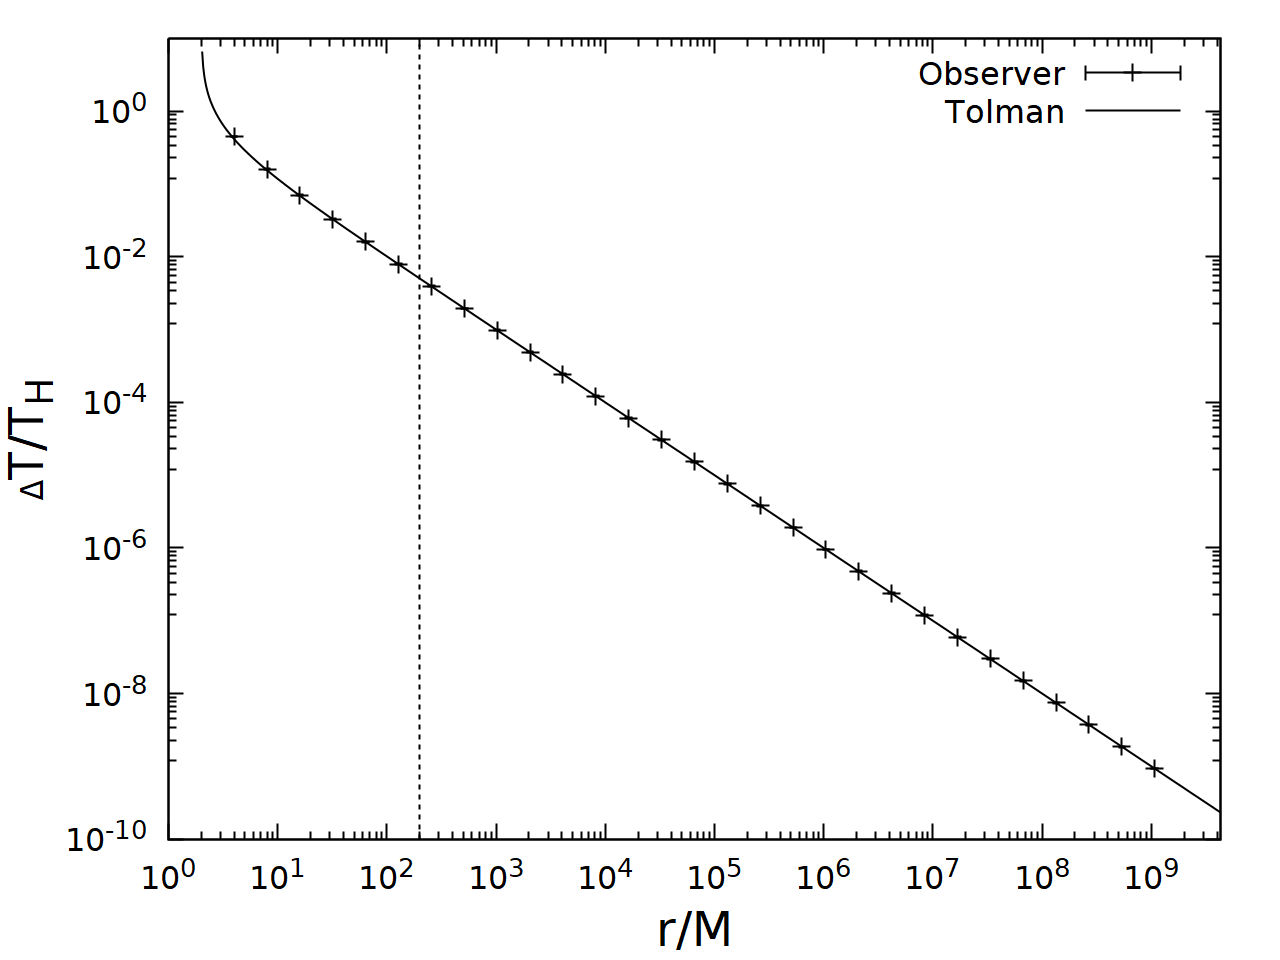
\includegraphics[width=\textwidth]{cpp/final/stat.png}
    \caption{Relative temperature shift}
  \end{subfigure}%
  \begin{subfigure}[h]{0.5\textwidth}
    \centering
    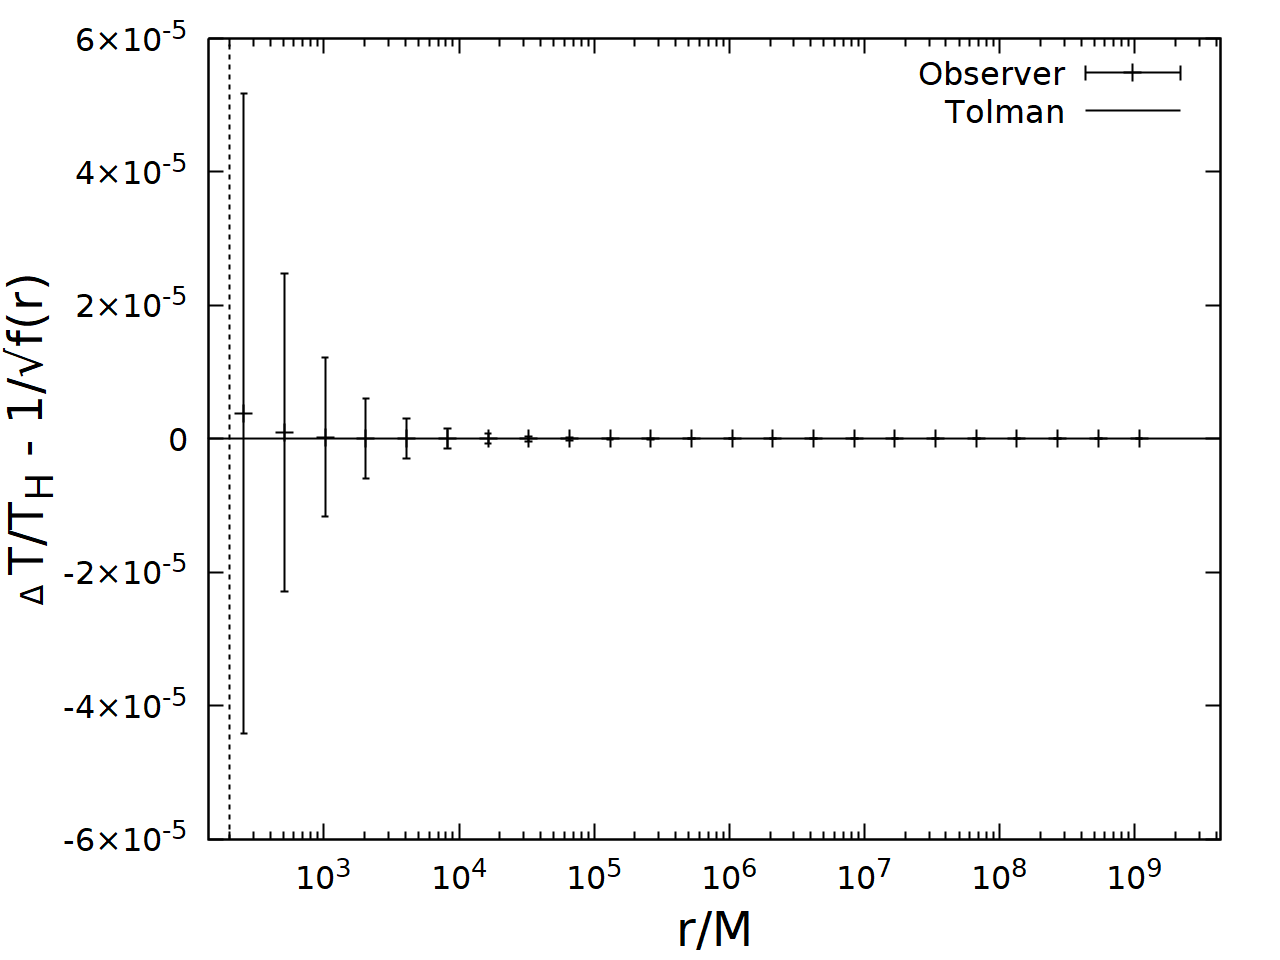
\includegraphics[width=\textwidth]{cpp/final/stat_tolman.png}
    \caption{Difference to Tolman relation}
  \end{subfigure}
  \caption[Static observer]{Static observer -- The relative temperature fits with Tolman-relation as shown in (a). In (b) the Tolman relation was subtracted. It matches with the Tolman relation within the numerical errors. Below the dotted line at \(r = 200M\) the approximation is not suitable.}
  \label{fig:bh_stat}
\end{figure}
 
\subsection{Circular observer}
\subsubsection{Before the collapse}
By Lemma \ref{lemma:killing} we know that a circular observer should see some excitations. Using our approximate form we can now calculate what he will actually measure. A circular observer is given by \(t = a\tau\), \(\varphi = B\tau\), \(r = \mathrm{const}\), \(\theta = \frac{\pi}{2}\)\footnote{Since the spacetime is spherically symmetric we can choose a coordinate system such that \(\theta = \frac{\pi}{2}\) and \(B>0\)}. The geodesic equation and \(\dot{\vb{x}}^2 = -1\) give constrains on the constants (see for example \cite{carroll})
\begin{align}
A^2 &= \frac{r}{r-3M}\\
B^2 &= \frac{1}{r^2}\frac{M}{r-3M}
\end{align}

The Wightman function evaluated on the curve is 
\begin{align}
D^+(\vb{x}(\tau), \vb{x}(\tau')) &= -\frac{1}{4\pi^2f(r)} \frac{1}{(A(\tau-\tau')-i\varepsilon)^2 - 2r_*^2 (1 - \cos{B(\tau-\tau')})}
\end{align}

We see that \(D^+\) only depends on \(\tau - \tau'\). So we can use the simplified formula \eqref{equ:qft_detector_final}. For this we need to find the poles in the lower half of \(D^+(\vb{x}(\tau),0)\) which means finding the roots of 

\begin{align}
0 &= A^2\tau^2 - 2r_*^2 (1 - \cos{B\tau})\\
0 &= \xi^2 x^2 - 2(1 - \cos{x})
\end{align}
where \(x = B\tau\) and \(\xi = \frac{A}{Br_*}\). 
Clearly \(\tau = 0\) is a root (which will lie in the upper half). Apart from that we have to differentiate between two cases:
\begin{itemize}
\item \(\xi < 1\): In this case there are two further roots on the real axis. The reason is that for \(\xi < 1\) (which is a very fast circular motion) the trajectory hits the Minkowski lightcone. But we know that this is not possible in the Schwarzschild-spacetime by the argumentation in Section \ref{sec:static_pole}. So we assume that this behaviour is due to our approximation and therefore exclude this case\footnote{Note that \(\xi < 1\) for a geodesic can only happen for \(r \lesssim 1.1 R\ind{S}\) which not far away from a black hole}.
\item \(\xi > 1\): This case represents slower motions. There are two more (first order) poles at \(\pm i x_0\) of whom one is in the lower half. 
\end{itemize}

The rate is given by eq. \eqref{equ:qft_detector_final}
\begin{align}
\dv{F_E}{\tau} &= \int_{-\infty}^\infty \dd{\tau} e^{-i E \tau} D^+(\vb{x}(\tau), \vb{x}(0))\\
	&= -\frac{1}{4\pi^2f(r)} \int_{-\infty}^\infty \dd{\tau} e^{-i E \tau} \frac{1}{A^2\tau^2 - 2r_*^2 (1 - \cos{B(\tau)})}\\
	&= -\frac{1}{4\pi^2 r_*^2 f(r) B} \int_{-\infty}^\infty \dd{x} e^{-i E x/B} \frac{1}{\xi^2 x^2 - 2 (1 - \cos{x})}\\
	&= \frac{i}{2\pi r_*^2 f(r) B}\mathrm{Res}\qty(e^{-i E x/B} \frac{1}{\xi^2 x^2 - 2 (1 - \cos{x})}, -ix_0)\\
	&= \frac{i}{2\pi r_*^2 f(r) B} e^{-E/B x_0} \lim_{x\to -i x_0} \frac{x + ix_0}{\xi^2 x^2 - 2 (1 - \cos{x})}\\
	&= \frac{1}{2\pi r_*^2 f(r) B} e^{-E/B x_0} \frac{1}{-2\xi^2 x_0 + 2 \sinh{x_0}}.
\end{align}

So basically a circular observer sees a exponentially falling energy distribution.

\subsubsection{After the collapse}
An observer on a circular orbit \(t = A \tau\) and \(\varphi = B\tau\) has the following thermal Wightman function:
\begin{align}
D^+_\beta(\vb{x}(\tau),\vb{x}(0)) &= -\frac{1}{4\beta^2 f(r)} \frac{1}{\sinh[2](\frac{\pi}{\beta}\sqrt{A^2\tau^2 - 2 r_*^2 (1-\cos{B\tau})})}
\end{align}

This function is problematic because expanding around zero yields:
\begin{align}
D^+_\beta(\vb{x}(\tau),\vb{x}(0)) &= -\frac{1}{4\pi^2 \tau^2} \frac{1}{f(r) A^2 - f(r)r_*^2 B^2} + \order*{\tau^0}\neq -\frac{1}{4\pi^2 \tau^2} + \order*{\tau^0}
\end{align}

Unfortunately the \(\tau^{-2}\) term has a different prefactor since we are only given \(\dot{\vb{x}}^2 = -f(r) A^2 + r^2 B^2 = -1\). However we know by Section \ref{sec:static_observers_thermal} that for every non approximate Wightman function on a trajectory this prefactor looks like \(-1/4\pi^2\). So this deviation is due to our approximation which is therefore only applicable if \(r^2 \approx f(r)r_*^2\). For \(r > 200 M\) the deviation is smaller than \(10 \%\). We will ignore smaller values of \(r\) for the interpretation of the results.

The main problem with the different prefactor is that the difference with another thermal Wightman function will remain divergent at \(\tau = 0\)\footnote{This difference must not be singular since we would like to integrate it numerically, see eq. \eqref{equ:app_num_formula}}. We can deal with this problem by replacing \(r_*^2\) by \(r^2/f(r)\) in the Wightman function
\begin{align}
D^+_\beta(\vb{x}(\tau),\vb{x}(0)) &= -\frac{1}{4\beta^2 f(r)} \frac{1}{\sinh[2](\frac{\pi}{\beta}\sqrt{A^2\tau^2 - 2 \frac{r^2}{f(r)} (1-\cos{B\tau})})}
\end{align}

This is possible because the approximation is only valid when the difference is negligible. Now we can determine the temperature shift according to Section \ref{sec:app_num}. The result is given in fig. \ref{fig:bh_circ}. One can see as long as our approximation is suitable (above the dotted line) the result fits to the Tolman relation. Again the difference between both lies inside the numerical errors.

\begin{figure}[h]
  \centering
  \begin{subfigure}[h]{0.5\textwidth}
    \centering
    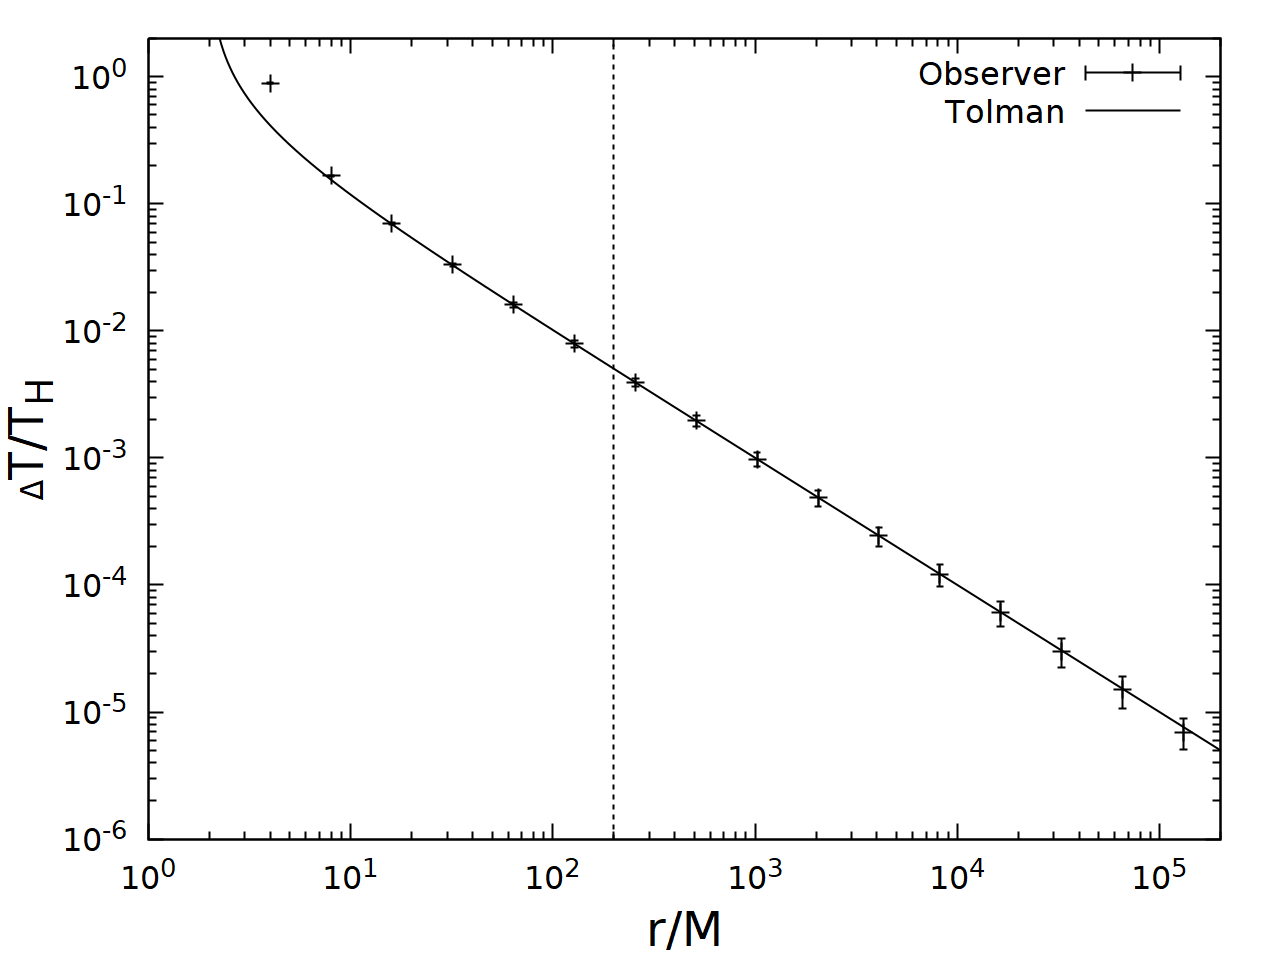
\includegraphics[width=\textwidth]{cpp/final/circ.png}
    \caption{Relative temperature shift}
  \end{subfigure}%
  \begin{subfigure}[h]{0.5\textwidth}
    \centering
    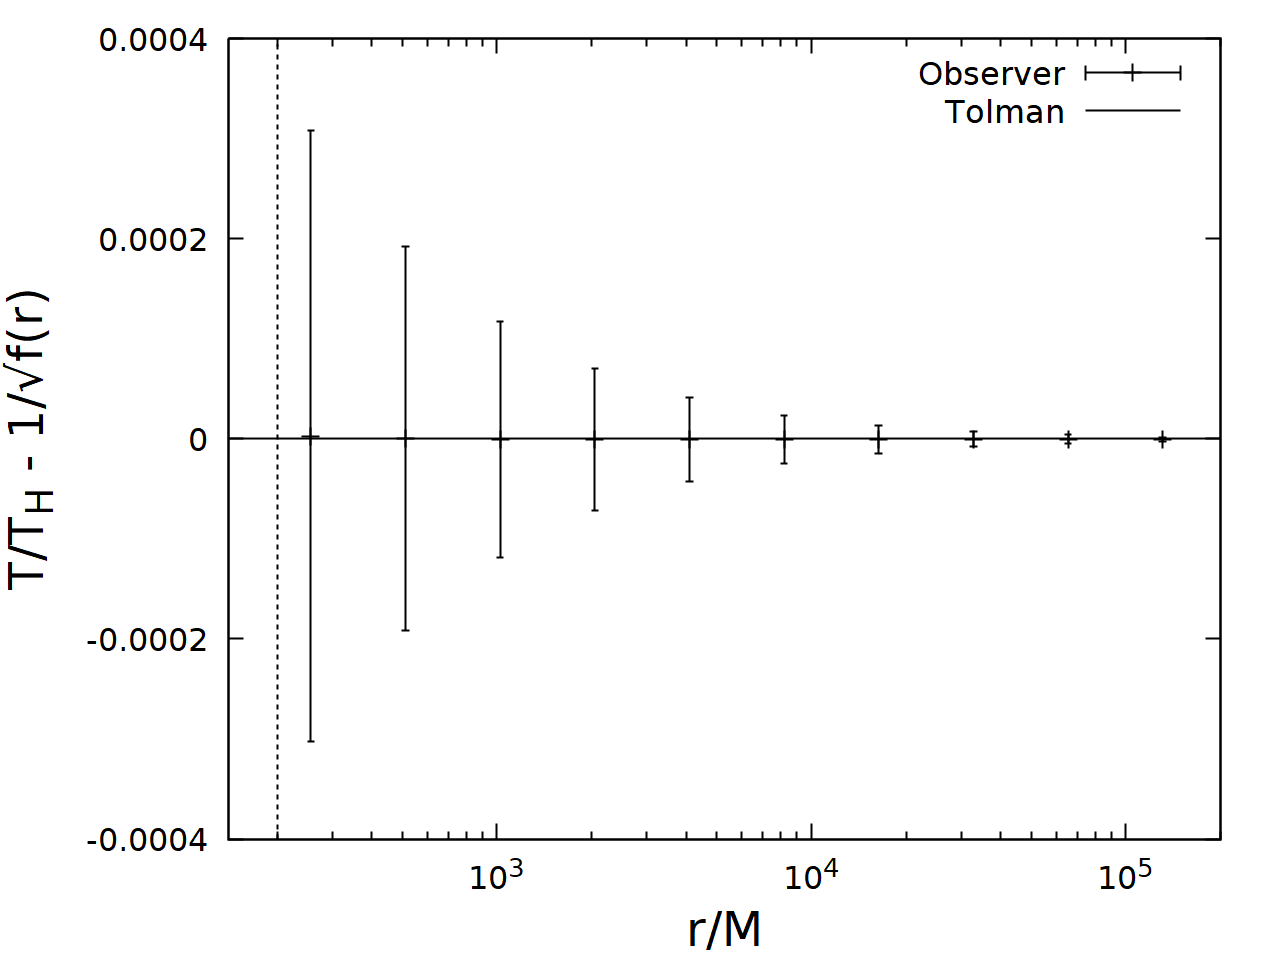
\includegraphics[width=\textwidth]{cpp/final/circ_tolman.png}
    \caption{Difference to Tolman relation}
  \end{subfigure}
  \caption[Circular observer]{Circular observer -- The relative temperature fits with Tolman-relation as shown in (a). In (b) the Tolman relation was subtracted. It matches with the Tolman relation within the numerical errors. Below the dotted line at \(r = 200M\) the approximation is not suitable.}
  \label{fig:bh_circ}
\end{figure} 

\subsection{Radial observer after the collapse}

We will restrict ourselves to the case of a freely falling observer that is dropped at infinity with zero velocity. This means \(E = f(r) \dot{t} = 1\). The geodesic equation and \(\dot{\vb{x}}^2 = -1\) result in the following trajectory \cite{weinstein}:
\begin{align}
r(\tau) &= \qty(-\frac{3}{2}\sqrt{2M} \qty(\tau - \tau_0))^\frac{2}{3}\\
t(\tau) &= \tau - \tau_0 - 3\tau_0 \qty(\frac{1}{x(\tau)} + \frac{1}{2}\ln \frac{x(\tau)-1}{x(\tau)+1})
\end{align}   

where \(x(\tau) = -\dot{r} = \qty(1-\frac{\tau}{\tau_0})^{-\frac{1}{3}}\) and \(\tau_0 = \frac{4M}{3}\)\footnote{\(\tau_0\) is chosen such that at \(\tau = 0\) the observer hits the event horizon.}. This is inserted in the thermal Wightman function \eqref{equ:bh_wightman_thermal} and the measured temperature is determined (see fig. \ref{fig:bh_rad}).

\begin{figure}[h]
  \centering
  \begin{subfigure}[h]{0.5\textwidth}
    \centering
    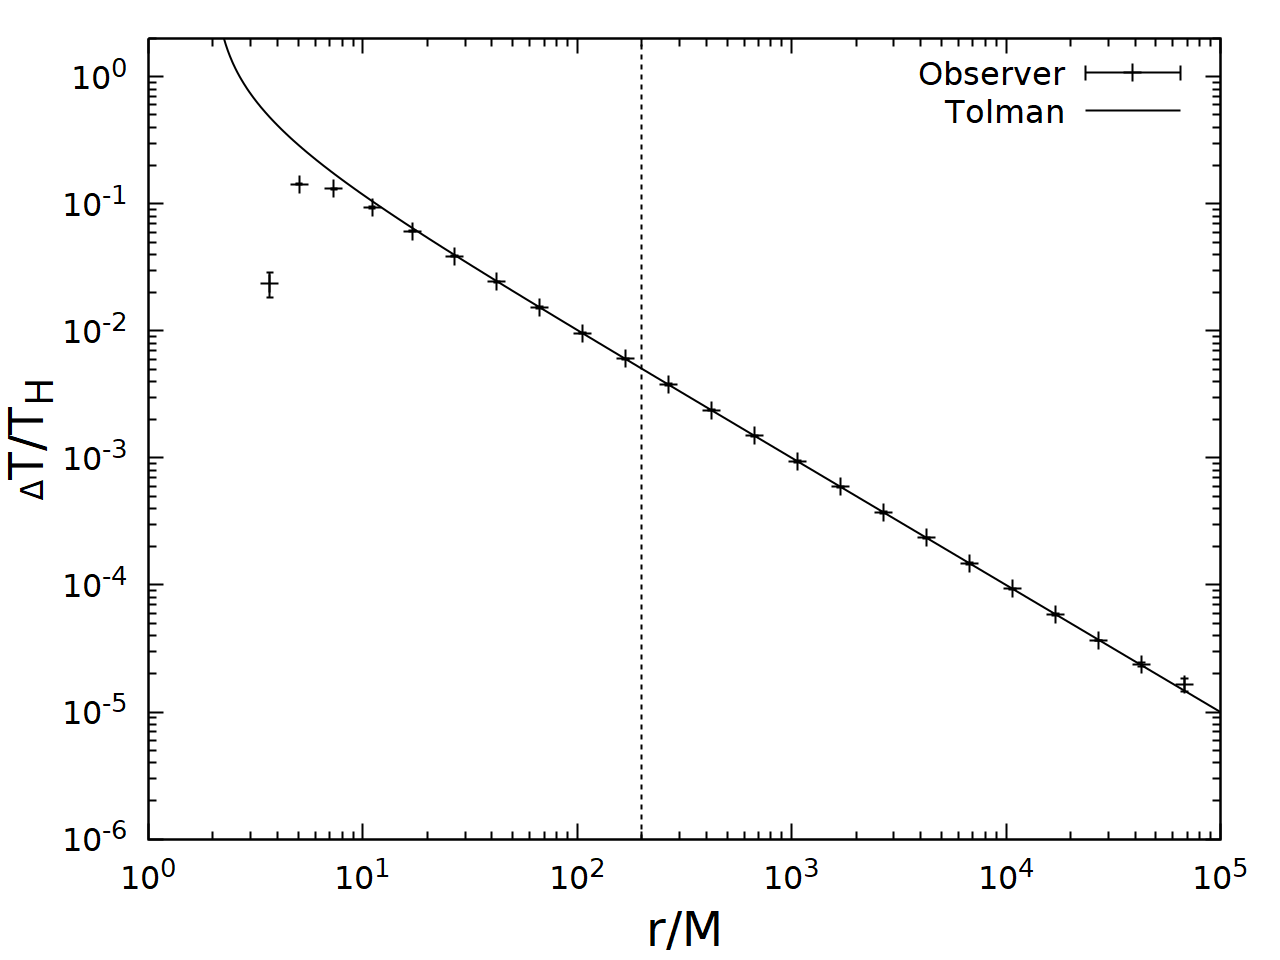
\includegraphics[width=\textwidth]{cpp/final/rad.png}
    \caption{Relative temperature shift}
  \end{subfigure}%
  \begin{subfigure}[h]{0.5\textwidth}
    \centering
    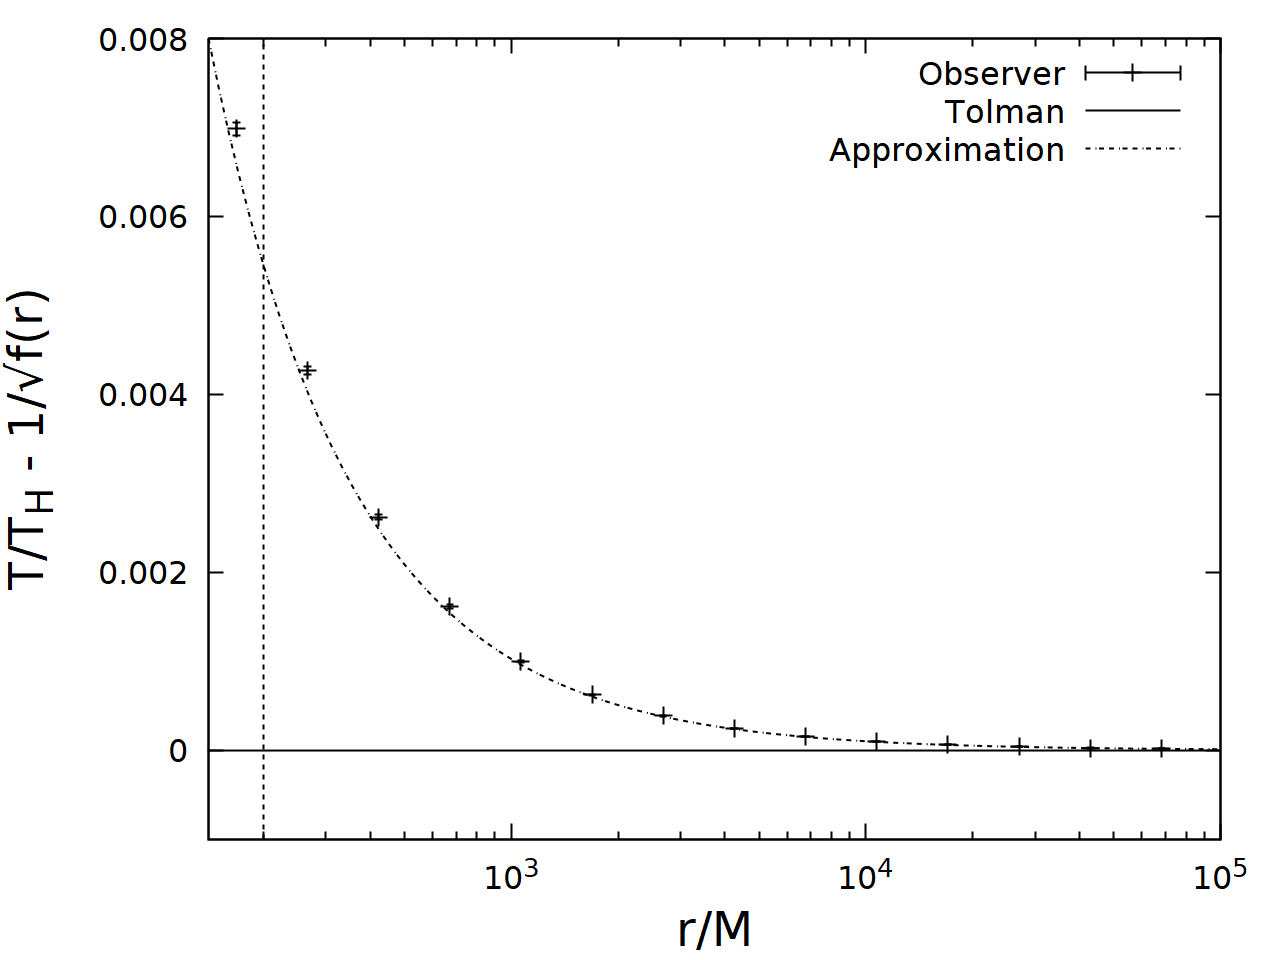
\includegraphics[width=\textwidth]{cpp/final/rad_tolman_error.png}
    \caption{Difference to Tolman relation}
  \end{subfigure}
  \caption[Radial infalling observer]{Radial infalling observer -- The relative temperature fits with Tolman-relation as shown in (a). In (b) the Tolman relation was subtracted. The difference is outside of the numerical errors even for radii \(r > 200 M\) (dotted vertical line). However the difference has the same order of magnitude of the estimated error caused by approximating the Wightman function (dotted curve).}
  \label{fig:bh_rad}
\end{figure}

The result again fits the Tolman relation. After subtracting the Tolman relation we find a difference much larger than the numerical errors. Note that the error bars only depict the numerical error, not the error done by approximating the Wightman function. In the last section we found that we can only use our Wightman function when \(\frac{r_*^2}{r^2} f(r) \approx 1\). We need to estimate the order of magnitude of the error caused by this approximation in order to show whether or not the difference in fig. \ref{fig:bh_rad} (b) is a significant deviation from the Tolman relation. We can give a (rough) estimate by applying the relative error done by the approximation on the Tolman relation, i.e. \(\frac{r_*^2}{r^2} f(r) \cdot \qty(\frac{1}{\sqrt{f(r)}} - 1)\). This is given as a dotted curve in fig. \ref{fig:bh_rad} (b). The calculated temperature deviation has about the same order of magnitude. This means that the difference could be completely due to our approximation. We will therefore be conservative and conclude that up to the errors of our method there is no temperature shift for an infalling observer.         
\chapter{Conclusion}
We showed properties of the Wightman function and the spectrum of an Unruh detector in a static spacetime. Using normal coordinates we were able to find that the singularity at \(\vb{x} = \vb{x}'\) will -- when evaluated on a curve -- give a second order pole \(-\frac{1}{4\pi^2 \tau^2}\) which is shifted to the upper half by a small regularisation \(\varepsilon\). This term does not contribute to the spectrum. We argued that apart from this singularity the Wightman function on any timelike curve will remain finite.

Moreover we found that in general in a static spacetime in the vacuum state a static observer does not encounter any particles. If the spacetime is in a thermal state with temperature \(T_0\) the observer sees a thermal spectrum with a different temperature according to the Tolman relation: \(T = \frac{T_0}{\sqrt{g_{tt}}}\). For an observer moving along a spatial killing vectorfield we found a condition when particles are encountered in the vacuum state which is independent of whether the trajectory is a geodesic or not. In particular, this means the particle spectrum is a global effect and cannot be treated in a local manner.    

We were able to apply these results to find an approximate form of the Wightman function in the outer Schwarzschild metric. This approximation is valid for \(r \gtrsim 200 M\). Using it we showed the general results from before explicitly: a static observer does not encounter any particles and a circular geodesic observer sees a non vanishing spectrum. Then we applied Hawking's result which states that after the collapse to a black hole the field is in a thermal state with \(\beta = 8\pi M\). A method to determine the temperature measured by different observers moving in this spacetime was developed and applied to static, circular and radial infalling observers. In all cases the temperature followed the Tolman relation. For static and circular observers there was no difference up to numerical errors. For radial observers we found a slight deviation outside the numerical errors. However this deviation has the same order of magnitude as expected by our approximation. Therefore a better approximation would be necessary to decide whether this is significant or not. For the time being we can only conclude that for all considered observers the temperature is given by the Tolman relation.    

We conclude our discussion by comparing the given results to those mentioned in the introduction. Both approaches also yield that the Tolman relation describes the temperature for static observers. In \cite{smerlak} (local treatment of the detector) a result is only stated explicitly for a circular observer which slightly differs from ours. But the difference has the same order of magnitude as the expected error through our approximation. So again here one would need a more exact Wightman function to find whether both results agree. The numerical approach in \cite{Hodgkinson} -- which is more similar to our method since it is also non local -- leads to an observed temperature given by the Tolman relation for circular observers which is consistent with our result.    

  

%------------------------------------------------------------------------------
% Add your chapters here - don't forget to also add them to \includeonly above
%%==============================================================================
\chapter{Introduction}
\label{sec:intro}
%==============================================================================

The introduction usually gives a few pages of introduction to the
whole subject, maybe even starting with the Greeks.

For more information on \LaTeX{} and the packages that are available
see for example the books of Kopka~\cite{kopka04} and Goossens et
al~\cite{goossens04}.

A lot of useful information on particle physics can be found in the
\enquote{Particle Data Book}~\cite{pdg2010}.

I have resisted the temptation to put a lot of definitions into the
file \texttt{thesis\_defs.sty}, as everyone has their own taste as
to what scheme they want to use for names.
However, a few examples are included to help you get started:
\begin{itemize}
\setlength{\itemsep}{0pt}\setlength{\parskip}{0pt}
\item cross-sections are measured in \si{\pb} and integrated
  luminosity in \si{\invpb};
\item the \KoS is an interesting particle;
\item the missing transverse momentum, \pTmiss, is often called
  missing transverse energy, even though it is calculated using a vector sum.
\end{itemize}
Note that the examples of units assume that you are using the
\textsf{siunitx} package.

It also is probably a good idea to include a few well formatted
references in the thesis skeleton. More detailed suggestions on what
citation types to use can be found in the thesis
guide~\cite{thesis-guide}:
\begin{itemize}
\item articles in refereed journals\cite{pdg2010,Aad:2010ey};
\item a book~\cite{Halzen:1984mc};
\item a PhD thesis~\cite{tlodd:2012} and a Diplom thesis~\cite{mergelmeyer:2011};
\item a collection of articles~\cite{lhc:vol1};
\item a conference note~\cite{ATLAS-CONF-2011-008};
\item a preprint~\cite{atlas:perf:2009} (you can also use
  \texttt{@online} or \texttt{@booklet}for such things);
\item something that is only available online~\cite{thesis-guide}.
\end{itemize}

At the end of the introduction it is normal to say briefly what comes
in the following chapters.

The lines at the end of this file are used by AUCTeX to specify which
is the master \LaTeX{} file, so that you can compile your thesis
directly within \texttt{emacs}.

%%% Local Variables: 
%%% mode: latex
%%% TeX-master: "../mythesis"
%%% End: 

% Uncomment the following command to get references per chapter.
% Put it inside the file or change \include to \input if you do not want the references
% on a separate page
% \printbibliography[heading=subbibliography]

%------------------------------------------------------------------------------
% Use biblatex for the bibliography
% Add bibliography to Table of Contents
% Comment out this command if your references are printed for each chapter.
\printbibliography
%[heading=bibintoc]

%------------------------------------------------------------------------------
% Include the following lines and comment out \printbibliography if
% you use BiBTeX for the bibliography.
% If you use biblatex package the files should be specified in the preamble.
% \KOMAoptions{toc=bibliography}
% {\raggedright
%   \bibliographystyle{refs/atlasBibStyleWithTitle.bst}
   % \bibliographystyle{unsrt}
   %\bibliography{./thesis_refs,../refs/standard_refs-bibtex}
% }

%------------------------------------------------------------------------------
\appendix
% \part*{Appendix}
% Add your appendices here - don't forget to also add them to \includeonly above
%%------------------------------------------------------------------------------
\chapter{Appendix}
\label{sec:app}
\begin{refsection}
%------------------------------------------------------------------------------

\section{Wightmanfunction in Minkowskispace}
\label{sec:app_minwightvac}
Using eq. \eqref{equ:wightman_modes} we can calculate the Wightman function:
\begin{align}
D^+(\vb{x},\vb{x}') &= \int \dd[3]{k} u_{\va{k}}(x) u_{\va{k}}^*(x')\\
	&= \int \frac{\dd[3]{k}}{(2\pi)^3}\, \frac{1}{2|\va{k}|} e^{- i |\va{k}| (t-t') + i \va{k} (\va{x}-\va{x}')}\\
	&\overset{\omega = |\va{k}|}{=} \int_0^\infty \int_{-1}^1 \frac{\omega^2 \dd{\omega}\dd{\cos{\theta}}}{(2\pi)^2}\, \cfrac{1}{2\omega} e^{- i \omega (t-t') + i \omega |\va{x}-\va{x}'| \cos{\theta}}\\
	&= \cfrac{1}{2 i |\va{x}-\va{x}'|}\int_0^\infty \frac{\dd{\omega}}{(2\pi)^2}\, e^{- i \omega (t-t')} \qty(e^{i\omega |\va{x}-\va{x}'|} - e^{-i\omega |\va{x}-\va{x}'|})
\end{align}

This oscillating integral does not converge. Therefore we will first calculate \(D^+(\vb{x},\vb{x}')\) for complex times by setting \(t \to t - i\varepsilon, \varepsilon > 0\) and then treating \(D^+(\vb{x},\vb{x}')\) as a distribution when setting \(\varepsilon \to 0\).

\begin{align}
D^+(\vb{x},\vb{x}') &= \cfrac{1}{2 i |\va{x}-\va{x}'|}\int_0^\infty \frac{\dd{\omega}}{(2\pi)^2}\, e^{- i \omega (t-t' - i\varepsilon - |\va{x}-\va{x}'|)} - e^{- i \omega (t-t' - i\varepsilon + |\va{x}-\va{x}'|)}\\
	&= -\cfrac{1}{2 i |\va{x}-\va{x}'|}\frac{1}{(2\pi)^2}\qty(\frac{i}{t-t' - i\varepsilon - |\va{x}-\va{x}'|} - \frac{i}{t-t' - i\varepsilon + |\va{x}-\va{x}'|})\\
	&= -\frac{1}{4\pi^2} \frac{1}{(t-t'-i\varepsilon)^2 - |\va{x}-\va{x}'|^2}
\end{align}

Alternatively one can achieve the form by first choosing a coordinate system such that \(\vb{x} = \tilde{t} \partial_0\) (as we will do for the thermal case) and then transforming it back (one has to be very careful with the \(\varepsilon\) here). \cite{davies} 

\section{Thermal Wigthman function in Minkowski space}
\label{sec:app_minwighttherm}
To calculate the thermal Wightman function we will restrict to the interior of the light cone (we will only need that). At a specific point choose the following coordinate system: First we will set \(\vb{x}' = 0\) and then choose a coordinate system such that \(\vb{x} = \tilde{t} \partial_0\). Here \(\tilde{t} = \pm \sqrt{-\vb{x}^2}\) with the upper sign for \(t > 0\) and the lower for \(t < 0\). In this coordinate system we can redo the calculation of the Wightman function and achieve
\begin{align}
D^+(\vb{x},0) = -\frac{1}{4\pi^2} \frac{1}{(\tilde{t} - i\varepsilon)^2}
\end{align} 

To find the thermal Wightmanfunction we to replace \(\tilde{t} \to \tilde{t} - i \beta n\) (see eq. \eqref{equ:qft_thermal}) and add all the contributions (note that inside the lightcone \(D^+ = D^{(1)}\))
\begin{align}
D^+_\beta(\vb{x},0) &= -\frac{1}{4\pi^2} \sum_{n=-\infty}^\infty \frac{1}{(\tilde{t} -i\beta n - i\varepsilon)^2}\\
	&= \frac{1}{4\pi^2\beta^2} \sum_{n=-\infty}^\infty \frac{1}{(- i \frac{\tilde{t}}{\beta} - n - \varepsilon)^2}\\
	&= \frac{1}{4\beta^2} \frac{1}{\sin[2](- i \pi \frac{\tilde{t}}{\beta} - \varepsilon)}\\
	&= -\frac{1}{4\beta^2} \frac{1}{\sinh[2](\frac{\pi}{\beta}(\tilde{t} - i\varepsilon))}
\end{align}

Here we used \(\sin[-2](\pi x) = \pi^{-2} \sum_n (x-n)^{-2}\) \cite{davies}. Now go back to the old frame and replace \(\tilde{t} = \pm \sqrt{-\vb{x}^2}\)
\begin{align}
D^+_\beta(\vb{x},\vb{x}') &= -\frac{1}{4\beta^2} \frac{1}{\sinh[2](\frac{\pi}{\beta}\qty(\pm \sqrt{(t-t')^2 - |\va{x}-\va{x}'|^2} - i\varepsilon))}\\
	&= -\frac{1}{4\beta^2} \frac{1}{\sinh[2](\frac{\pi}{\beta}\sqrt{(t-t'-i\varepsilon)^2 - |\va{x}-\va{x}'|^2})}. \text{\cite{davies}}
\end{align}

\section{The Unruh-Detector}
\label{sec:app_unruh}
\todo{shorten?}
Our treatment of such a detector will follow Birrell and Davies \cite{davies}.
One describes a detector by a operator \(m(\tau)\) which couples to the field via a interaction term \(c\cdot m(\tau) \phi(\vb{x}(\tau))\), where \(c\) is small and \(\vb{x}(\tau)\) is the trajectory of the detector. For \(\tau \to -\infty\) the detector is in the groundstate \(\ket*{E_0}\) and the field is in the vacuum state \(\ket*{0}\). The detector develops with time according to \(m(\tau) = e^{i H_0 \tau} m(0) e^{-i H_0 \tau}\) with \(H_0 \ket*{E} = E\ket*{E}\).

We would like to calculate the probability that the detector detects a particle with energy \(E\). Since \(c\) is small one can use first order perturbation theory where the transition amplitude to another state \(\ket*{E,\psi}\) at time \(\tau\) is given by
\begin{align}
Q_{\ket*{E_0,0}\to\ket*{E,\psi}}(\tau) &= i c \bra*{E,\psi} \int_{-\infty}^\tau m(\tau') \phi(\vb{x}(\tau'))\dd{\tau'}\ket*{E_0,0}\\
	&= i c \bra*{E,\psi} \int_{-\infty}^\tau e^{i H_0 \tau'} m(0) e^{-i H_0 \tau'} \phi(\vb{x}(\tau'))\dd{\tau'}\ket*{E_0,0}\\
	&= i c \bra*{\psi} \int_{-\infty}^\tau e^{i E \tau'} \bra{E}m(0)\ket{E_0}  e^{-i E_0 \tau'} \phi(\vb{x}(\tau'))\dd{\tau'}\ket*{0}\\
	&= i c \bra{E}m(0)\ket{E_0} \int_{-\infty}^\tau e^{i (E-E_0) \tau'} \bra*{\psi}\phi(\vb{x}(\tau'))\ket*{0}\dd{\tau'}
\end{align}

The transition probability is \(P_{\ket{E_0,0}\to\ket{E,\psi}}(\tau) = |Q_{\ket{E_0,0}\to\ket{E,\psi}}(\tau)|^2\). But since we are only interested in the state of the detector we sum over all field configurations:
\begin{align}
P_E(\tau) &:= \sum_{i} P_{\ket*{E_0,0}\to\ket*{E,\psi_i}}(\tau) = \sum_{i}  |Q_{\ket*{E_0,0}\to\ket*{E,\psi}}(\tau)|^2\\
		  &= c^2 |\bra*{E}m(0)\ket*{E_0}|^2 F_{E-E_0}(\tau)\\
\text{with}\,F_E(\tau) &= \sum_{i}\qty|\int_{-\infty}^\tau e^{i E \tau} \bra*{\psi_i}\phi(\vb{x}(\tau'))\ket*{0}\dd{\tau'}|^2\\
	&= \sum_{i} \int_{-\infty}^\tau e^{-i E \tau''} \bra*{0}\phi(\vb{x}(\tau''))\dd{\tau''}\ket*{\psi_i}\bra*{\psi_i}\int_{-\infty}^\tau e^{i E \tau'} \phi(\vb{x}(\tau'))\ket*{0}\dd{\tau'}\\
	&= \int_{-\infty}^\tau\dd{\tau'} \int_{-\infty}^\tau \dd{\tau''} e^{-i E (\tau''-\tau')} \bra*{0}\phi(\vb{x}(\tau'')) \phi(\vb{x}(\tau'))\ket*{0}\\ 
	&= \int_{-\infty}^\tau\dd{\tau'} \int_{-\infty}^\tau \dd{\tau''} e^{-i E (\tau''-\tau')} D^+(\vb{x}(\tau''), \vb{x}(\tau'))
\end{align}

Here we introduced the Wightman function \(D^+(\vb{x},\vb{x}') = \bra*{0}\phi(\vb{x}) \phi(\vb{x}')\ket*{0}\). The probability splits in a product of two parts. The first one only depends on the model of the detector while the second part only depends on the trajectory. We will therefore interpret the (so called detector response) function \(F_E(\tau)\) as the distribution of energy excitations (or particles) as 'seen' by an observer on the trajectory \(\vb{x}(\tau)\).

The transition rate is then given by:
\begin{align}
\dv{F_E}{\tau} &= \int_{-\infty}^\tau \dd{\tau''} e^{-i E (\tau''-\tau)} D^+(\vb{x}(\tau''), \vb{x}(\tau)) + \int_{-\infty}^\tau \dd{\tau'} e^{-i E (\tau-\tau')} D^+(\vb{x}(\tau), \vb{x}(\tau'))\\
&= 2 \mathrm{Re} \int_{-\infty}^0 \dd{\tilde{\tau}} e^{-i E \tilde{\tau}} D^+(\vb{x}(\tilde{\tau} + \tau), \vb{x}(\tau))
\end{align}

since \(D^+(\vb{x},\vb{x}')^* = D^+(\vb{x}',\vb{x})\). For the special case that the Wightman function does only depend on the difference of the \(\tau\text{'s}\), i.e. \(D^+(\vb{x}(\tau_1 + \tau'),\vb{x}(\tau_2 + \tau')) = D^+(\vb{x}(\tau_1),\vb{x}(\tau_2))\) one can simplify this further:

\begin{align}
\dv{F_E}{\tau} &=  \int_{-\infty}^0 \dd{\tilde{\tau}} e^{-i E \tilde{\tau}} D^+(\vb{x}(\tilde{\tau} + \tau), \vb{x}(\tau)) + \int_{0}^\infty \dd{\tilde{\tau}} e^{- i E \tilde{\tau}} D^+(\vb{x}(\tau), \vb{x}(\tau - \tilde{\tau}))\\
	&= \int_{-\infty}^0 \dd{\tilde{\tau}} e^{-i E \tilde{\tau}} D^+(\vb{x}(\tilde{\tau} + \tau), \vb{x}(\tau)) + \int_{0}^\infty \dd{\tilde{\tau}} e^{- i E \tilde{\tau}} D^+(\vb{x}(\tau  + \tilde{\tau}), \vb{x}(\tau))\\
	&= \int_{-\infty}^\infty \dd{\tilde{\tau}} e^{-i E \tilde{\tau}} D^+(\vb{x}(\tilde{\tau} + \tau), \vb{x}(\tau)) = \int_{-\infty}^\infty \dd{\tilde{\tau}} e^{-i E \tilde{\tau}} D^+(\vb{x}(\tilde{\tau}), \vb{x}(0))
\end{align}

The rate is the Fourier transform of the Wightman function and is independent of \(\tau\).\cite{davies}

\section{Wightman function in normal coordinates}
\label{sec:app_normal}
Fix \(\vb{x}' = 0\). The metric in normal coordinates then looks like \cite{davies}:
\begin{align}
g_{ij} &= \delta_{ij} - \frac{1}{3} R_{iajb} x^a x^b + \order{x^3}
\end{align}

Since the metric is given to the second order we will also expand other quantities\footnote{Note that one can raise and lower indices with \(\delta_{ij}\) if one is neglecting \(\order*{x^2}\).}
\begin{align}
g^{ij} &= \delta^{ij} + \frac{1}{3} R^{i\;j}_{\;a\;b} x^a x^b + \order{x^3}\\
\partial_i g^{ij} &= -\frac{1}{3} R^j_{\;i} x^i + \order{x^2} = -\frac{1}{3} R_{ji} x^i + \order{x^2}\\
g = \det g_{ij} &= 1 - \frac{1}{3} R_{ij} x^i x^j + \order{x^3}\\  
\frac{1}{g}\partial_i g &= -\frac{2}{3} R_{ij} x^j + \order{x^2}\\
\beta &= a + b_i x^i + \frac{1}{2} c_{ij} x^i x^j + \order{x^3}
\end{align}

\subsection{Solutions of the Klein-Gordon-equation}

The Klein-Gordon-equation is given by
\begin{align}
0 &= \nabla_\mu\nabla^\mu\phi = -\frac{1}{\sqrt{\beta g}} \partial_t \qty(\sqrt{\beta g} \frac{1}{\beta} \partial_t \phi) + \frac{1}{\sqrt{\beta g}} \partial_i \qty(\sqrt{\beta g} g^{ij} \partial_j \phi)\\
&= -\frac{1}{\beta} \partial_t^2 \phi + \frac{1}{\sqrt{\beta g}} \partial_i \qty(\sqrt{\beta g})  g^{ij} \partial_j \phi +  \qty(\partial_i g^{ij}) \partial_j \phi + g^{ij} \partial_i \partial_j \phi\\
&= -\frac{1}{\beta} \partial_t^2 \phi + \frac{1}{2\beta g} \partial_i \qty(\beta g) g^{ij} \partial_j \phi +  \qty(\partial_i g^{ij}) \partial_j \phi + g^{ij} \partial_i \partial_j \phi\\
\partial_t^2 \phi &= \frac{\partial_i\beta}{2} g^{ij} \partial_j \phi + \frac{\beta \partial_i g}{2g} g^{ij} \partial_j \phi + \beta \qty(\partial_i g^{ij}) \partial_j \phi + \beta g^{ij} \partial_i \partial_j \phi\\
&= \frac{1}{2} \qty(b_i + c_{ik} x^k) \partial_i \phi - \frac{a}{3} R_{ik} x^k \partial_i \phi - \frac{a}{3} R_{ik} x^k \partial_ i\phi + \qty(a + b_k x^k) \partial_i \partial_i \phi + \order{x^2}\\
&= \frac{1}{2} \qty(b_i + c_{ik} x^k) \partial_i \phi - \frac{2a}{3} R_{ik} x^k \partial_i \phi + \qty(a + b_k x^k) \partial_i \partial_i \phi + \order{x^2}
\end{align}

To solve these equations make the ansatz \(\tilde{u}_{\va{k}}(\vb{x}) = \exp(-i\omega t + i k_i x^i + i \frac{1}{2} k_a B^{a}_{ij}(\va{k}) x^i x^j + i\order*{x^3})\) and separate the different orders:

\begin{align}
-\omega^2 &= \frac{1}{2} \qty(b_i + c_{ik} x^k) i \qty(k_i + k_a B^a_{ik} x^k) - \frac{2a}{3} R_{ik} x^k i k_i\notag\\
&\,+ \qty(a + b_k x^k) \qty(i k_a B^a_{ii} - \qty(k_i + k_a B^a_{ik} x^k)\qty(k_i + k_b B^b_{il} x^l)) + \order{x^2}\\
-\omega^2 &= \frac{1}{2}i b_i k_i + a i k_a B^a_{ii} - a k_ik_i\\
0 &= ik_a\qty(\frac{1}{2} b_i B^a_{ik} + \frac{1}{2} c_{ak} - \frac{2a}{3} R_{ak} + b_k B^a_{ii}) - 2 a k_i k_a B^a_{ik} - b_k k_i k_i 
\end{align}

If we demand that all parameters should be real then we have 8 equations for 18 free parameters of \(B^a_{ij}\)\footnote{Note that \(B^a_{ij}\) is symmetric in \(i, j\).}. We could now fix some more properties of \(B\) but it is not necessary for our argumentation. Note that the dispersion relation now reads \(\omega = \sqrt{a} \qty|\va{k}|\).

\subsection{Normalising the modes}
Next we need to find the right normalisation of the modes. Since we can't integrate our modes over the whole spacetime we will use the CCR to find the right normalisation\footnote{This works because the CCR are only valid in the right normalisation}. So expand \(\phi(\vb{x}) = \int \frac{\dd[3]{k}}{\sqrt{2\pi}^3} \frac{1}{\sqrt{2\omega N_{\va{k}}}}\tilde{u}_{\va{k}}(\vb{x}) a_{\va{k}} + \frac{1}{\sqrt{2\omega N_{\va{k}}}} \tilde{u}_{\va{k}}(\vb{x})^* a_{\va{k}}^\dagger\) and calculate the CCR for a surface \(t = \mathrm{const.}\):

\begin{align}
[\phi(\vb{x}), \phi(0)] &= \int \frac{\dd[3]{k}}{(2\pi)^3} \frac{1}{2\omega N_{\va{k}}}\tilde{u}_{\va{k}}(\vb{x}) \tilde{u}_{\va{k}}(0)^*  - \frac{1}{2\omega N_{\va{k}}}\tilde{u}_{\va{k}}(\vb{x})^* \tilde{u}_{\va{k}}(0)\\
	&= i \int \frac{\dd[3]{k}}{(2\pi)^3} \frac{1}{2\omega N_{\va{k}}} e^{i \va{k}\va{x} + \order*{x^2}} - \frac{1}{2\omega N_{\va{k}}}e^{-i \va{k}\va{x} + \order*{x^2}} \overset{!}{=} 0\\
%
[\phi(\vb{x}), \sqrt{g} \partial_0 \phi(0)] &= i \int \frac{\dd[3]{k}}{(2\pi)^3} \frac{1}{2N_{\va{k}}}\tilde{u}_{\va{k}}(\vb{x}) \tilde{u}_{\va{k}}(0)^* + \frac{1}{2N_{\va{k}}}\tilde{u}_{\va{k}}(\vb{x})^* \tilde{u}_{\va{k}}(0) + \order{x^2}\\
   &= i \int \frac{\dd[3]{k}}{(2\pi)^3} \frac{1}{2N_{\va{k}}} e^{i \va{k}\va{x} + \order*{x^2}} + \frac{1}{2N_{\va{k}}}e^{-i \va{k}\va{x} + \order*{x^2}} + \order{x^2}\\
   &\overset{!}{=} i \delta^3(\va{x}) = i \int \frac{\dd[3]{k}}{(2\pi)^3} e^{i \va{k}\va{x}}\\
%   
[\sqrt{g} \partial_0 \phi(\vb{x}), \sqrt{g} \partial_0 \phi(0)] &= \int \frac{\dd[3]{k}}{(2\pi)^3} \frac{\omega}{2 N_{\va{k}}}\tilde{u}_{\va{k}}(\vb{x}) \tilde{u}_{\va{k}}(0)^* - \frac{\omega}{2 N_{\va{k}}}\tilde{u}_{\va{k}}(\vb{x})^* \tilde{u}_{\va{k}}(0)  + \order{x^2}\\
	&= i \int \frac{\dd[3]{k}}{(2\pi)^3} \frac{\omega}{2 N_{\va{k}}} e^{i \va{k}\va{x} + \order*{x^2}} - \frac{\omega}{2 N_{\va{k}}}e^{-i \va{k}\va{x} + \order*{x^2}} + \order{x^2} \overset{!}{=} 0
\end{align}

Since \(e^{i \va{k}\va{x}}\) is a basis we find:
\begin{align}
\frac{1}{2\omega N_{\va{k}}} - \frac{1}{2\omega N_{-\va{k}}} &= 0\\
\frac{1}{2N_{\va{k}}} + \frac{1}{2N_{-\va{k}}} &= 1\\
\frac{\omega}{2N_{\va{k}}} - \frac{\omega}{2 N_{-\va{k}}} &= 0
\end{align}

This system of equations is only solved for \(N_{\va{k}} = 1\) and so the normalised modes are
\begin{align}
u_{\va{k}} &= \frac{1}{\sqrt{2\pi}^3 \sqrt{2\omega}} e^{-i\omega t + i\va{k}\va{x} + \order*{x^2}}\\
	&= \frac{1}{\sqrt{2\pi}^3 \sqrt{2\omega}} e^{-i\omega t + i\va{k}\va{x}} \qty(1 + \order{x^2})
\end{align}

So up to linear order we achieve the plane wave modes as in Minkowski space. Therefore the Wightman function is also the equivalent and given by
\begin{align}
D^+(\vb{x},0) = - \frac{1}{4\pi^2} \frac{1}{a(t-i\varepsilon)^2 - |\va{x}|^2} + \order{x^2}
\end{align}

\section{Determination of the temperature}
\label{sec:app_num}
In chapter \ref{sec:bh} we need to find the temperature that an observer will see on the basis of the energy spectrum. The energy spectrum is basically given by a Fourier-like transform of \(D^+\) evaluated along the curve (see eq. \eqref{equ:qft_detector_partial} and \eqref{equ:qft_detector_final}). 
\subsection{Idea}
Imaging an observer equipped with an Unruh-detector on a trajectory in the Schwarzschild metric. By eq. \eqref{equ:static_thermal_observer_general} he expects some thermal spectrum together with some corrections. These corrections could either shift the observed temperature or could be part of the non thermal spectrum. However he won't be able to distinguish which part of the spectrum is thermal or not. So to determine the temperature he will fit a thermal spectrum into the observed spectrum, i.e. find a value \(\beta\) such that the following minimizes: 
\begin{align}
\int_0^\infty \dd{E} \qty(\dv{F_E}{\tau} - \frac{1}{2\pi} \frac{E}{e^{\beta E}-1})^2 \to \mathrm{min}
\end{align}

We will use this measurement process to define the temperature observed \todo{understandable} on a trajectory. To minimize this we don't need to calculate the spectrum first, we can equivalently directly minimize the difference of \(D^+\) and the thermal Wightman function in Minkowski space

\begin{align}
D_\beta\upd{M}(\tau') = -\frac{1}{4\beta^2} \frac{1}{\sinh[2](\frac{\pi}{\beta} \tau')}
\end{align}

corresponding to \(\beta\)\footnote{This is due to the Plancherel theorem which states that the integral over the square of a function equals the integral over the square of its Fourier transform.}:

\begin{align}
\int_{-\infty}^0 \dd{\tau'} \qty(D^+(\vb{x}(\tau + \tau'), \vb{x}(\tau)) - D_\beta\upd{M}(\tau'))^2 \to \mathrm{min}
\end{align} 

We expect the temperature shift to be small compared to the Hawking temperature \(\beta\ind{H} = 8\pi M\) (and indeed this will be the case). So we can do a Taylor expansion of the thermal Wightman function around \(\beta\ind{H}\)\footnote{Note that we are expanding around the fixed Hawking temperature and not around the position dependent Tolman temperature \(\beta\ind{static} = \sqrt{f(r)}\beta\ind{H}\). This is useful to compare the observed temperatures.} This yields to

\begin{align}
D_\beta\upd{M}(\tau') &\approx D_{\beta\ind{H}}\upd{M}(\tau') + \frac{\Delta\beta}{\beta\ind{H}} \frac{\sinh(\frac{\pi}{\beta\ind{H}} \tau') - \frac{\pi}{\beta\ind{H}} \tau' \cosh(\frac{\pi}{\beta\ind{H}} \tau')}{2\beta\ind{H}^2 \sinh[3](\frac{\pi}{\beta\ind{H}} \tau')} \\
	&=: D_{\beta\ind{H}}\upd{M}(\tau') + \alpha g(\tau')
\end{align}

We would like to compute \(\alpha = \frac{\Delta\beta}{\beta\ind{H}} = \frac{\beta - \beta\ind{H}}{\beta\ind{H}}\). This is easily done because we can find the minimum by differentiating w.r.t. \(\alpha\):
\begin{align}
\int_{-\infty}^0 &\dd{\tau'} \qty(D^+(\vb{x}(\tau + \tau'), \vb{x}(\tau)) - D_{\beta\ind{H}}\upd{M}(\tau') - \alpha g(\tau'))^2 \to \mathrm{min}\\
\alpha &= \frac{\int_{-\infty}^0 \dd{\tau'} \qty(D^+(\vb{x}(\tau + \tau'), \vb{x}(\tau)) - D_{\beta\ind{H}}\upd{M}(\tau'))\cdot g(\tau')}{\int_{-\infty}^0 \dd{\tau'} g(\tau')^2}\\
	&=: \frac{\int_{-\infty}^0 \dd{\tau'} h(\tau')\cdot g(\tau')}{\int_{-\infty}^0 \dd{\tau'} g(\tau')^2}
\label{equ:app_num_formula}
\end{align}

The integral over \(g^2\) can be calculated ones and yields \(I_g = \int_{-\infty}^0 \dd{\tau'} g(\tau')^2 = \frac{15 - \pi^2}{92160 \pi^4} M^{-3} \approx 5.7149\cdot 10^{-7} M^{-3}\)\todo{explain?}. In the diagrams we will not plot \(\alpha\) but rather \(-\alpha = \Delta T/T\ind{H}\).

\subsection{Error estimation}
The other integral \(I = \int_{-\infty}^0 \dd{\tau'} h(\tau')g(\tau')\) is evaluated numerically using the trapezoidal rule (see for example \cite{ron}). Since we cannot integrate the infinite range \((-\infty,0)\) with this method we will integrate over a finite range \((\tau_1,\tau_2)\)\footnote{Note that all \(\tau\) are negative.}. In order to get a meaningful result we need to estimate the errors. There are basically 3 sources of errors: the lower and upper integration limit and the error by the method itself.

For big absolute values of \(\tau'\) we can replace the \(\sinh\) and \(\cosh\) in \(g\) by an exponential function:
\begin{align}
g(\tau') &\approx \frac{1 - \frac{\pi}{\beta\ind{H}} \tau'}{2\beta\ind{H}^2} \exp(2\frac{\pi}{\beta\ind{H}} \tau')\\
	&\approx -\frac{\pi}{2 \beta\ind{H}^3} \tau' \exp(2\frac{\pi}{\beta\ind{H}} \tau')
\label{equ:app_num_g_asymptotic}
\end{align}

Integrating this from \(-\infty\) to \(\tau_1\) yields\todo{check}:
\begin{align}
\int_{-\infty}^{\tau_1} g(\tau') &= \frac{1}{4\beta\ind{H}}\qty(\frac{-\tau_1}{\beta_H} + \frac{1}{2\pi}) \exp(2\frac{\pi}{\beta\ind{H}} \tau_1)\\
&\approx \frac{\beta\ind{H}}{2\pi} g(\tau_1)
\end{align}

Since \(h\) will drop to zero we can assume an upper bound of the error for sufficiently small \(\tau_1\) by

\begin{align}
\Delta I_1 \approx \frac{\beta\ind{H}}{2\pi} |g(\tau_1)h(\tau_1)| 
\end{align}

Another error arises from the fact\todo{anders?} that around zero \(h\) is the (finite) difference of two divergent functions. Evaluating the function is therefore afflicted with increasing sampling errors when approaching zero. Since we cannot control those errors we will stop integrating at \(\tau_2 \lesssim 0\). When we assume that the function is nearly constant on the small interval we can add the missing contribution \(g(\tau_2)h(\tau_2)\cdot |\tau_2|\). However this will lead to an error which we estimate generously by the expected amount of the contribution:
\begin{align}
\Delta I_2 \approx |g(\tau_2)h(\tau_2) \tau_2| \approx |g(0)h(0) \tau_2|
\end{align}

The last contribution comes from the error of the method used. For the trapezoidal method this error is given by (\(\Delta\tau\) is the stepwidth)\cite{ron}
\begin{align}
\Delta I\ind{trapez} = \frac{\Delta\tau^2}{12} (\tau_2-\tau_1) |(h\cdot g)''(\chi)| 
\end{align}

where \(\chi\) is some value in the interval \((\tau_1,\tau_2)\). Since the \(h\cdot g\) will asymptotically drop to zero at least exponentially the second derivative will also drop. We are therefore interested in the curvature nearby \(\chi \approx \tau_2 \approx 0\). In fact we will use the second derivative at zero to estimate the error:
\begin{align}
\Delta I\ind{trapez} \approx \frac{\Delta\tau^2}{12} (\tau_2-\tau_1) |(h\cdot g)''(0)|
\label{equ:app_num_dtrapez}
\end{align}

Recall that we minimized \(\int (h - \alpha g)^2\) and therefore expect \(h \approx \alpha g\). So \((h\cdot g)''(0) \approx (\alpha g^2)''(0)\) that inserting into \eqref{equ:app_num_formula} yields\todo{check}
\begin{align}
\Delta I\ind{trapez} \approx \alpha \frac{\Delta\tau^2}{12} (\tau_2-\tau_1) \frac{2 \pi^2}{45 \beta^6}
\end{align} 

To compare the order of magnitude of the different error contributions we will replace \(h \approx \alpha g\), use the asymptotic form of \(g\) in \eqref{equ:app_num_g_asymptotic} and express all quantities in units of the mass of the star (i.e. set \(M = 1\))
\begin{align}
\Delta I_1[M^{-3}] &= 4 |g(\tau_1)h(\tau_1)| \approx \alpha \frac{1}{524288\pi^4} \tau_1[M]^2 \exp(\frac{1}{2} \tau_1[M])\\
\Delta I_2[M^{-3}] &= |g(0) h(0) \tau_2| \approx \alpha \frac{1}{36 \beta^4} |\tau_2| = \alpha\frac{1}{147456 \pi^4} |\tau_2[M]|\\
\Delta I\ind{trapez}[M^{-3}] &= \alpha \frac{\Delta\tau^2}{12} (\tau_2-\tau_1) \frac{2 \pi^2}{45 \beta^6} \approx \alpha \Delta\tau[M]^2 (\tau_2[M]-\tau_1[M]) \frac{1}{70778880 \pi^4}
\end{align}

Apart from the \(\tau_2\) we can minimize the errors by choosing sufficient values for \(\tau_1\) and \(\Delta\tau\). If we set 
\begin{align}
\label{equ:app_num_cond_1}
\Delta \tau[M] &\ll 1/(\tau_2[M]-\tau_1[M]])\\
\Delta \tau[M] &\ll |\tau_2[M]|
\end{align}
 the contribution of \(\Delta I\ind{trapez}\) is neglectable compared to \(\Delta I_2\). If we further set \(\tau_1\) such that 
\begin{align}
\tau_1[M]^2 \exp(\frac{1}{2} \tau_1[M]) \ll |\tau_2[M]|
\label{equ:app_num_cond_2}
\end{align} 
we can also neglect \(\Delta I_1\). So the dominant error contribution will come from \(\Delta I_2 = |g(0) h(0) \tau_2|\). This error is -- as the value -- divided by \(I_g\) to achieve the error on \(\alpha\) which is then given in the diagrams as errorbars.

For computing those diagrams the parameters in tab. \ref{tab:app_num_params} were used. One can easily check that they fulfil relations \eqref{equ:app_num_cond_1} - \eqref{equ:app_num_cond_2}. It was necessary to adjust \(\tau_2\) for circular observers because the numerical errors increased with increasing \(r\). For the other observers \(g\cdot h\) became thinner with increasing \(r\) till the sampling errors dominated. Therefore it was not possible to use this algorithm for arbitrary high radii.
\begin{table}
\centering
\caption[Integration parameters]{Parameters used for numerical integration: integration from \(\tau_1\) to \(\tau_2\) using \(\Delta\tau\) as stepwidth.}
\label{tab:app_num_params}
\begin{tabular}{cccc}
\toprule
Observer & \(\tau_1[M]\) & \(\tau_2[M]\) & \(\Delta\tau[M]\)\\
\midrule
static & \(-40\) & \(-0.1\) &  \(0.0001\)\\
circular & \(-40\) & \(-(\log_2(r)/10)^2\) &  \(0.0001\)\\
radial & \(-40\) & \(-0.1\) &  \(0.0001\)\\
\bottomrule
\end{tabular}
\end{table}

\printbibliography[heading=subbibliography]

\end{refsection}
%------------------------------------------------------------------------------
\chapter{Appendix}
\label{sec:app}
\begin{refsection}
%------------------------------------------------------------------------------

\section{Wightmanfunction in Minkowskispace}
\label{sec:app_minwightvac}
Using eq. \eqref{equ:wightman_modes} we can calculate the Wightman function:
\begin{align}
D^+(\vb{x},\vb{x}') &= \int \dd[3]{k} u_{\va{k}}(x) u_{\va{k}}^*(x')\\
	&= \int \frac{\dd[3]{k}}{(2\pi)^3}\, \frac{1}{2|\va{k}|} e^{- i |\va{k}| (t-t') + i \va{k} (\va{x}-\va{x}')}\\
	&\overset{\omega = |\va{k}|}{=} \int_0^\infty \int_{-1}^1 \frac{\omega^2 \dd{\omega}\dd{\cos{\theta}}}{(2\pi)^2}\, \cfrac{1}{2\omega} e^{- i \omega (t-t') + i \omega |\va{x}-\va{x}'| \cos{\theta}}\\
	&= \cfrac{1}{2 i |\va{x}-\va{x}'|}\int_0^\infty \frac{\dd{\omega}}{(2\pi)^2}\, e^{- i \omega (t-t')} \qty(e^{i\omega |\va{x}-\va{x}'|} - e^{-i\omega |\va{x}-\va{x}'|})
\end{align}

This oscillating integral does not converge. Therefore we will first calculate \(D^+(\vb{x},\vb{x}')\) for complex times by setting \(t \to t - i\varepsilon, \varepsilon > 0\) and then treating \(D^+(\vb{x},\vb{x}')\) as a distribution when setting \(\varepsilon \to 0\).

\begin{align}
D^+(\vb{x},\vb{x}') &= \cfrac{1}{2 i |\va{x}-\va{x}'|}\int_0^\infty \frac{\dd{\omega}}{(2\pi)^2}\, e^{- i \omega (t-t' - i\varepsilon - |\va{x}-\va{x}'|)} - e^{- i \omega (t-t' - i\varepsilon + |\va{x}-\va{x}'|)}\\
	&= -\cfrac{1}{2 i |\va{x}-\va{x}'|}\frac{1}{(2\pi)^2}\qty(\frac{i}{t-t' - i\varepsilon - |\va{x}-\va{x}'|} - \frac{i}{t-t' - i\varepsilon + |\va{x}-\va{x}'|})\\
	&= -\frac{1}{4\pi^2} \frac{1}{(t-t'-i\varepsilon)^2 - |\va{x}-\va{x}'|^2}
\end{align}

Alternatively one can achieve the form by first choosing a coordinate system such that \(\vb{x} = \tilde{t} \partial_0\) (as we will do for the thermal case) and then transforming it back (one has to be very careful with the \(\varepsilon\) here). \cite{davies} 

\section{Thermal Wigthman function in Minkowski space}
\label{sec:app_minwighttherm}
To calculate the thermal Wightman function we will restrict to the interior of the light cone (we will only need that). At a specific point choose the following coordinate system: First we will set \(\vb{x}' = 0\) and then choose a coordinate system such that \(\vb{x} = \tilde{t} \partial_0\). Here \(\tilde{t} = \pm \sqrt{-\vb{x}^2}\) with the upper sign for \(t > 0\) and the lower for \(t < 0\). In this coordinate system we can redo the calculation of the Wightman function and achieve
\begin{align}
D^+(\vb{x},0) = -\frac{1}{4\pi^2} \frac{1}{(\tilde{t} - i\varepsilon)^2}
\end{align} 

To find the thermal Wightmanfunction we to replace \(\tilde{t} \to \tilde{t} - i \beta n\) (see eq. \eqref{equ:qft_thermal}) and add all the contributions (note that inside the lightcone \(D^+ = D^{(1)}\))
\begin{align}
D^+_\beta(\vb{x},0) &= -\frac{1}{4\pi^2} \sum_{n=-\infty}^\infty \frac{1}{(\tilde{t} -i\beta n - i\varepsilon)^2}\\
	&= \frac{1}{4\pi^2\beta^2} \sum_{n=-\infty}^\infty \frac{1}{(- i \frac{\tilde{t}}{\beta} - n - \varepsilon)^2}\\
	&= \frac{1}{4\beta^2} \frac{1}{\sin[2](- i \pi \frac{\tilde{t}}{\beta} - \varepsilon)}\\
	&= -\frac{1}{4\beta^2} \frac{1}{\sinh[2](\frac{\pi}{\beta}(\tilde{t} - i\varepsilon))}
\end{align}

Here we used \(\sin[-2](\pi x) = \pi^{-2} \sum_n (x-n)^{-2}\) \cite{davies}. Now go back to the old frame and replace \(\tilde{t} = \pm \sqrt{-\vb{x}^2}\)
\begin{align}
D^+_\beta(\vb{x},\vb{x}') &= -\frac{1}{4\beta^2} \frac{1}{\sinh[2](\frac{\pi}{\beta}\qty(\pm \sqrt{(t-t')^2 - |\va{x}-\va{x}'|^2} - i\varepsilon))}\\
	&= -\frac{1}{4\beta^2} \frac{1}{\sinh[2](\frac{\pi}{\beta}\sqrt{(t-t'-i\varepsilon)^2 - |\va{x}-\va{x}'|^2})}. \text{\cite{davies}}
\end{align}

\section{The Unruh-Detector}
\label{sec:app_unruh}
\todo{shorten?}
Our treatment of such a detector will follow Birrell and Davies \cite{davies}.
One describes a detector by a operator \(m(\tau)\) which couples to the field via a interaction term \(c\cdot m(\tau) \phi(\vb{x}(\tau))\), where \(c\) is small and \(\vb{x}(\tau)\) is the trajectory of the detector. For \(\tau \to -\infty\) the detector is in the groundstate \(\ket*{E_0}\) and the field is in the vacuum state \(\ket*{0}\). The detector develops with time according to \(m(\tau) = e^{i H_0 \tau} m(0) e^{-i H_0 \tau}\) with \(H_0 \ket*{E} = E\ket*{E}\).

We would like to calculate the probability that the detector detects a particle with energy \(E\). Since \(c\) is small one can use first order perturbation theory where the transition amplitude to another state \(\ket*{E,\psi}\) at time \(\tau\) is given by
\begin{align}
Q_{\ket*{E_0,0}\to\ket*{E,\psi}}(\tau) &= i c \bra*{E,\psi} \int_{-\infty}^\tau m(\tau') \phi(\vb{x}(\tau'))\dd{\tau'}\ket*{E_0,0}\\
	&= i c \bra*{E,\psi} \int_{-\infty}^\tau e^{i H_0 \tau'} m(0) e^{-i H_0 \tau'} \phi(\vb{x}(\tau'))\dd{\tau'}\ket*{E_0,0}\\
	&= i c \bra*{\psi} \int_{-\infty}^\tau e^{i E \tau'} \bra{E}m(0)\ket{E_0}  e^{-i E_0 \tau'} \phi(\vb{x}(\tau'))\dd{\tau'}\ket*{0}\\
	&= i c \bra{E}m(0)\ket{E_0} \int_{-\infty}^\tau e^{i (E-E_0) \tau'} \bra*{\psi}\phi(\vb{x}(\tau'))\ket*{0}\dd{\tau'}
\end{align}

The transition probability is \(P_{\ket{E_0,0}\to\ket{E,\psi}}(\tau) = |Q_{\ket{E_0,0}\to\ket{E,\psi}}(\tau)|^2\). But since we are only interested in the state of the detector we sum over all field configurations:
\begin{align}
P_E(\tau) &:= \sum_{i} P_{\ket*{E_0,0}\to\ket*{E,\psi_i}}(\tau) = \sum_{i}  |Q_{\ket*{E_0,0}\to\ket*{E,\psi}}(\tau)|^2\\
		  &= c^2 |\bra*{E}m(0)\ket*{E_0}|^2 F_{E-E_0}(\tau)\\
\text{with}\,F_E(\tau) &= \sum_{i}\qty|\int_{-\infty}^\tau e^{i E \tau} \bra*{\psi_i}\phi(\vb{x}(\tau'))\ket*{0}\dd{\tau'}|^2\\
	&= \sum_{i} \int_{-\infty}^\tau e^{-i E \tau''} \bra*{0}\phi(\vb{x}(\tau''))\dd{\tau''}\ket*{\psi_i}\bra*{\psi_i}\int_{-\infty}^\tau e^{i E \tau'} \phi(\vb{x}(\tau'))\ket*{0}\dd{\tau'}\\
	&= \int_{-\infty}^\tau\dd{\tau'} \int_{-\infty}^\tau \dd{\tau''} e^{-i E (\tau''-\tau')} \bra*{0}\phi(\vb{x}(\tau'')) \phi(\vb{x}(\tau'))\ket*{0}\\ 
	&= \int_{-\infty}^\tau\dd{\tau'} \int_{-\infty}^\tau \dd{\tau''} e^{-i E (\tau''-\tau')} D^+(\vb{x}(\tau''), \vb{x}(\tau'))
\end{align}

Here we introduced the Wightman function \(D^+(\vb{x},\vb{x}') = \bra*{0}\phi(\vb{x}) \phi(\vb{x}')\ket*{0}\). The probability splits in a product of two parts. The first one only depends on the model of the detector while the second part only depends on the trajectory. We will therefore interpret the (so called detector response) function \(F_E(\tau)\) as the distribution of energy excitations (or particles) as 'seen' by an observer on the trajectory \(\vb{x}(\tau)\).

The transition rate is then given by:
\begin{align}
\dv{F_E}{\tau} &= \int_{-\infty}^\tau \dd{\tau''} e^{-i E (\tau''-\tau)} D^+(\vb{x}(\tau''), \vb{x}(\tau)) + \int_{-\infty}^\tau \dd{\tau'} e^{-i E (\tau-\tau')} D^+(\vb{x}(\tau), \vb{x}(\tau'))\\
&= 2 \mathrm{Re} \int_{-\infty}^0 \dd{\tilde{\tau}} e^{-i E \tilde{\tau}} D^+(\vb{x}(\tilde{\tau} + \tau), \vb{x}(\tau))
\end{align}

since \(D^+(\vb{x},\vb{x}')^* = D^+(\vb{x}',\vb{x})\). For the special case that the Wightman function does only depend on the difference of the \(\tau\text{'s}\), i.e. \(D^+(\vb{x}(\tau_1 + \tau'),\vb{x}(\tau_2 + \tau')) = D^+(\vb{x}(\tau_1),\vb{x}(\tau_2))\) one can simplify this further:

\begin{align}
\dv{F_E}{\tau} &=  \int_{-\infty}^0 \dd{\tilde{\tau}} e^{-i E \tilde{\tau}} D^+(\vb{x}(\tilde{\tau} + \tau), \vb{x}(\tau)) + \int_{0}^\infty \dd{\tilde{\tau}} e^{- i E \tilde{\tau}} D^+(\vb{x}(\tau), \vb{x}(\tau - \tilde{\tau}))\\
	&= \int_{-\infty}^0 \dd{\tilde{\tau}} e^{-i E \tilde{\tau}} D^+(\vb{x}(\tilde{\tau} + \tau), \vb{x}(\tau)) + \int_{0}^\infty \dd{\tilde{\tau}} e^{- i E \tilde{\tau}} D^+(\vb{x}(\tau  + \tilde{\tau}), \vb{x}(\tau))\\
	&= \int_{-\infty}^\infty \dd{\tilde{\tau}} e^{-i E \tilde{\tau}} D^+(\vb{x}(\tilde{\tau} + \tau), \vb{x}(\tau)) = \int_{-\infty}^\infty \dd{\tilde{\tau}} e^{-i E \tilde{\tau}} D^+(\vb{x}(\tilde{\tau}), \vb{x}(0))
\end{align}

The rate is the Fourier transform of the Wightman function and is independent of \(\tau\).\cite{davies}

\section{Wightman function in normal coordinates}
\label{sec:app_normal}
Fix \(\vb{x}' = 0\). The metric in normal coordinates then looks like \cite{davies}:
\begin{align}
g_{ij} &= \delta_{ij} - \frac{1}{3} R_{iajb} x^a x^b + \order{x^3}
\end{align}

Since the metric is given to the second order we will also expand other quantities\footnote{Note that one can raise and lower indices with \(\delta_{ij}\) if one is neglecting \(\order*{x^2}\).}
\begin{align}
g^{ij} &= \delta^{ij} + \frac{1}{3} R^{i\;j}_{\;a\;b} x^a x^b + \order{x^3}\\
\partial_i g^{ij} &= -\frac{1}{3} R^j_{\;i} x^i + \order{x^2} = -\frac{1}{3} R_{ji} x^i + \order{x^2}\\
g = \det g_{ij} &= 1 - \frac{1}{3} R_{ij} x^i x^j + \order{x^3}\\  
\frac{1}{g}\partial_i g &= -\frac{2}{3} R_{ij} x^j + \order{x^2}\\
\beta &= a + b_i x^i + \frac{1}{2} c_{ij} x^i x^j + \order{x^3}
\end{align}

\subsection{Solutions of the Klein-Gordon-equation}

The Klein-Gordon-equation is given by
\begin{align}
0 &= \nabla_\mu\nabla^\mu\phi = -\frac{1}{\sqrt{\beta g}} \partial_t \qty(\sqrt{\beta g} \frac{1}{\beta} \partial_t \phi) + \frac{1}{\sqrt{\beta g}} \partial_i \qty(\sqrt{\beta g} g^{ij} \partial_j \phi)\\
&= -\frac{1}{\beta} \partial_t^2 \phi + \frac{1}{\sqrt{\beta g}} \partial_i \qty(\sqrt{\beta g})  g^{ij} \partial_j \phi +  \qty(\partial_i g^{ij}) \partial_j \phi + g^{ij} \partial_i \partial_j \phi\\
&= -\frac{1}{\beta} \partial_t^2 \phi + \frac{1}{2\beta g} \partial_i \qty(\beta g) g^{ij} \partial_j \phi +  \qty(\partial_i g^{ij}) \partial_j \phi + g^{ij} \partial_i \partial_j \phi\\
\partial_t^2 \phi &= \frac{\partial_i\beta}{2} g^{ij} \partial_j \phi + \frac{\beta \partial_i g}{2g} g^{ij} \partial_j \phi + \beta \qty(\partial_i g^{ij}) \partial_j \phi + \beta g^{ij} \partial_i \partial_j \phi\\
&= \frac{1}{2} \qty(b_i + c_{ik} x^k) \partial_i \phi - \frac{a}{3} R_{ik} x^k \partial_i \phi - \frac{a}{3} R_{ik} x^k \partial_ i\phi + \qty(a + b_k x^k) \partial_i \partial_i \phi + \order{x^2}\\
&= \frac{1}{2} \qty(b_i + c_{ik} x^k) \partial_i \phi - \frac{2a}{3} R_{ik} x^k \partial_i \phi + \qty(a + b_k x^k) \partial_i \partial_i \phi + \order{x^2}
\end{align}

To solve these equations make the ansatz \(\tilde{u}_{\va{k}}(\vb{x}) = \exp(-i\omega t + i k_i x^i + i \frac{1}{2} k_a B^{a}_{ij}(\va{k}) x^i x^j + i\order*{x^3})\) and separate the different orders:

\begin{align}
-\omega^2 &= \frac{1}{2} \qty(b_i + c_{ik} x^k) i \qty(k_i + k_a B^a_{ik} x^k) - \frac{2a}{3} R_{ik} x^k i k_i\notag\\
&\,+ \qty(a + b_k x^k) \qty(i k_a B^a_{ii} - \qty(k_i + k_a B^a_{ik} x^k)\qty(k_i + k_b B^b_{il} x^l)) + \order{x^2}\\
-\omega^2 &= \frac{1}{2}i b_i k_i + a i k_a B^a_{ii} - a k_ik_i\\
0 &= ik_a\qty(\frac{1}{2} b_i B^a_{ik} + \frac{1}{2} c_{ak} - \frac{2a}{3} R_{ak} + b_k B^a_{ii}) - 2 a k_i k_a B^a_{ik} - b_k k_i k_i 
\end{align}

If we demand that all parameters should be real then we have 8 equations for 18 free parameters of \(B^a_{ij}\)\footnote{Note that \(B^a_{ij}\) is symmetric in \(i, j\).}. We could now fix some more properties of \(B\) but it is not necessary for our argumentation. Note that the dispersion relation now reads \(\omega = \sqrt{a} \qty|\va{k}|\).

\subsection{Normalising the modes}
Next we need to find the right normalisation of the modes. Since we can't integrate our modes over the whole spacetime we will use the CCR to find the right normalisation\footnote{This works because the CCR are only valid in the right normalisation}. So expand \(\phi(\vb{x}) = \int \frac{\dd[3]{k}}{\sqrt{2\pi}^3} \frac{1}{\sqrt{2\omega N_{\va{k}}}}\tilde{u}_{\va{k}}(\vb{x}) a_{\va{k}} + \frac{1}{\sqrt{2\omega N_{\va{k}}}} \tilde{u}_{\va{k}}(\vb{x})^* a_{\va{k}}^\dagger\) and calculate the CCR for a surface \(t = \mathrm{const.}\):

\begin{align}
[\phi(\vb{x}), \phi(0)] &= \int \frac{\dd[3]{k}}{(2\pi)^3} \frac{1}{2\omega N_{\va{k}}}\tilde{u}_{\va{k}}(\vb{x}) \tilde{u}_{\va{k}}(0)^*  - \frac{1}{2\omega N_{\va{k}}}\tilde{u}_{\va{k}}(\vb{x})^* \tilde{u}_{\va{k}}(0)\\
	&= i \int \frac{\dd[3]{k}}{(2\pi)^3} \frac{1}{2\omega N_{\va{k}}} e^{i \va{k}\va{x} + \order*{x^2}} - \frac{1}{2\omega N_{\va{k}}}e^{-i \va{k}\va{x} + \order*{x^2}} \overset{!}{=} 0\\
%
[\phi(\vb{x}), \sqrt{g} \partial_0 \phi(0)] &= i \int \frac{\dd[3]{k}}{(2\pi)^3} \frac{1}{2N_{\va{k}}}\tilde{u}_{\va{k}}(\vb{x}) \tilde{u}_{\va{k}}(0)^* + \frac{1}{2N_{\va{k}}}\tilde{u}_{\va{k}}(\vb{x})^* \tilde{u}_{\va{k}}(0) + \order{x^2}\\
   &= i \int \frac{\dd[3]{k}}{(2\pi)^3} \frac{1}{2N_{\va{k}}} e^{i \va{k}\va{x} + \order*{x^2}} + \frac{1}{2N_{\va{k}}}e^{-i \va{k}\va{x} + \order*{x^2}} + \order{x^2}\\
   &\overset{!}{=} i \delta^3(\va{x}) = i \int \frac{\dd[3]{k}}{(2\pi)^3} e^{i \va{k}\va{x}}\\
%   
[\sqrt{g} \partial_0 \phi(\vb{x}), \sqrt{g} \partial_0 \phi(0)] &= \int \frac{\dd[3]{k}}{(2\pi)^3} \frac{\omega}{2 N_{\va{k}}}\tilde{u}_{\va{k}}(\vb{x}) \tilde{u}_{\va{k}}(0)^* - \frac{\omega}{2 N_{\va{k}}}\tilde{u}_{\va{k}}(\vb{x})^* \tilde{u}_{\va{k}}(0)  + \order{x^2}\\
	&= i \int \frac{\dd[3]{k}}{(2\pi)^3} \frac{\omega}{2 N_{\va{k}}} e^{i \va{k}\va{x} + \order*{x^2}} - \frac{\omega}{2 N_{\va{k}}}e^{-i \va{k}\va{x} + \order*{x^2}} + \order{x^2} \overset{!}{=} 0
\end{align}

Since \(e^{i \va{k}\va{x}}\) is a basis we find:
\begin{align}
\frac{1}{2\omega N_{\va{k}}} - \frac{1}{2\omega N_{-\va{k}}} &= 0\\
\frac{1}{2N_{\va{k}}} + \frac{1}{2N_{-\va{k}}} &= 1\\
\frac{\omega}{2N_{\va{k}}} - \frac{\omega}{2 N_{-\va{k}}} &= 0
\end{align}

This system of equations is only solved for \(N_{\va{k}} = 1\) and so the normalised modes are
\begin{align}
u_{\va{k}} &= \frac{1}{\sqrt{2\pi}^3 \sqrt{2\omega}} e^{-i\omega t + i\va{k}\va{x} + \order*{x^2}}\\
	&= \frac{1}{\sqrt{2\pi}^3 \sqrt{2\omega}} e^{-i\omega t + i\va{k}\va{x}} \qty(1 + \order{x^2})
\end{align}

So up to linear order we achieve the plane wave modes as in Minkowski space. Therefore the Wightman function is also the equivalent and given by
\begin{align}
D^+(\vb{x},0) = - \frac{1}{4\pi^2} \frac{1}{a(t-i\varepsilon)^2 - |\va{x}|^2} + \order{x^2}
\end{align}

\section{Determination of the temperature}
\label{sec:app_num}
In chapter \ref{sec:bh} we need to find the temperature that an observer will see on the basis of the energy spectrum. The energy spectrum is basically given by a Fourier-like transform of \(D^+\) evaluated along the curve (see eq. \eqref{equ:qft_detector_partial} and \eqref{equ:qft_detector_final}). 
\subsection{Idea}
Imaging an observer equipped with an Unruh-detector on a trajectory in the Schwarzschild metric. By eq. \eqref{equ:static_thermal_observer_general} he expects some thermal spectrum together with some corrections. These corrections could either shift the observed temperature or could be part of the non thermal spectrum. However he won't be able to distinguish which part of the spectrum is thermal or not. So to determine the temperature he will fit a thermal spectrum into the observed spectrum, i.e. find a value \(\beta\) such that the following minimizes: 
\begin{align}
\int_0^\infty \dd{E} \qty(\dv{F_E}{\tau} - \frac{1}{2\pi} \frac{E}{e^{\beta E}-1})^2 \to \mathrm{min}
\end{align}

We will use this measurement process to define the temperature observed \todo{understandable} on a trajectory. To minimize this we don't need to calculate the spectrum first, we can equivalently directly minimize the difference of \(D^+\) and the thermal Wightman function in Minkowski space

\begin{align}
D_\beta\upd{M}(\tau') = -\frac{1}{4\beta^2} \frac{1}{\sinh[2](\frac{\pi}{\beta} \tau')}
\end{align}

corresponding to \(\beta\)\footnote{This is due to the Plancherel theorem which states that the integral over the square of a function equals the integral over the square of its Fourier transform.}:

\begin{align}
\int_{-\infty}^0 \dd{\tau'} \qty(D^+(\vb{x}(\tau + \tau'), \vb{x}(\tau)) - D_\beta\upd{M}(\tau'))^2 \to \mathrm{min}
\end{align} 

We expect the temperature shift to be small compared to the Hawking temperature \(\beta\ind{H} = 8\pi M\) (and indeed this will be the case). So we can do a Taylor expansion of the thermal Wightman function around \(\beta\ind{H}\)\footnote{Note that we are expanding around the fixed Hawking temperature and not around the position dependent Tolman temperature \(\beta\ind{static} = \sqrt{f(r)}\beta\ind{H}\). This is useful to compare the observed temperatures.} This yields to

\begin{align}
D_\beta\upd{M}(\tau') &\approx D_{\beta\ind{H}}\upd{M}(\tau') + \frac{\Delta\beta}{\beta\ind{H}} \frac{\sinh(\frac{\pi}{\beta\ind{H}} \tau') - \frac{\pi}{\beta\ind{H}} \tau' \cosh(\frac{\pi}{\beta\ind{H}} \tau')}{2\beta\ind{H}^2 \sinh[3](\frac{\pi}{\beta\ind{H}} \tau')} \\
	&=: D_{\beta\ind{H}}\upd{M}(\tau') + \alpha g(\tau')
\end{align}

We would like to compute \(\alpha = \frac{\Delta\beta}{\beta\ind{H}} = \frac{\beta - \beta\ind{H}}{\beta\ind{H}}\). This is easily done because we can find the minimum by differentiating w.r.t. \(\alpha\):
\begin{align}
\int_{-\infty}^0 &\dd{\tau'} \qty(D^+(\vb{x}(\tau + \tau'), \vb{x}(\tau)) - D_{\beta\ind{H}}\upd{M}(\tau') - \alpha g(\tau'))^2 \to \mathrm{min}\\
\alpha &= \frac{\int_{-\infty}^0 \dd{\tau'} \qty(D^+(\vb{x}(\tau + \tau'), \vb{x}(\tau)) - D_{\beta\ind{H}}\upd{M}(\tau'))\cdot g(\tau')}{\int_{-\infty}^0 \dd{\tau'} g(\tau')^2}\\
	&=: \frac{\int_{-\infty}^0 \dd{\tau'} h(\tau')\cdot g(\tau')}{\int_{-\infty}^0 \dd{\tau'} g(\tau')^2}
\label{equ:app_num_formula}
\end{align}

The integral over \(g^2\) can be calculated ones and yields \(I_g = \int_{-\infty}^0 \dd{\tau'} g(\tau')^2 = \frac{15 - \pi^2}{92160 \pi^4} M^{-3} \approx 5.7149\cdot 10^{-7} M^{-3}\)\todo{explain?}. In the diagrams we will not plot \(\alpha\) but rather \(-\alpha = \Delta T/T\ind{H}\).

\subsection{Error estimation}
The other integral \(I = \int_{-\infty}^0 \dd{\tau'} h(\tau')g(\tau')\) is evaluated numerically using the trapezoidal rule (see for example \cite{ron}). Since we cannot integrate the infinite range \((-\infty,0)\) with this method we will integrate over a finite range \((\tau_1,\tau_2)\)\footnote{Note that all \(\tau\) are negative.}. In order to get a meaningful result we need to estimate the errors. There are basically 3 sources of errors: the lower and upper integration limit and the error by the method itself.

For big absolute values of \(\tau'\) we can replace the \(\sinh\) and \(\cosh\) in \(g\) by an exponential function:
\begin{align}
g(\tau') &\approx \frac{1 - \frac{\pi}{\beta\ind{H}} \tau'}{2\beta\ind{H}^2} \exp(2\frac{\pi}{\beta\ind{H}} \tau')\\
	&\approx -\frac{\pi}{2 \beta\ind{H}^3} \tau' \exp(2\frac{\pi}{\beta\ind{H}} \tau')
\label{equ:app_num_g_asymptotic}
\end{align}

Integrating this from \(-\infty\) to \(\tau_1\) yields\todo{check}:
\begin{align}
\int_{-\infty}^{\tau_1} g(\tau') &= \frac{1}{4\beta\ind{H}}\qty(\frac{-\tau_1}{\beta_H} + \frac{1}{2\pi}) \exp(2\frac{\pi}{\beta\ind{H}} \tau_1)\\
&\approx \frac{\beta\ind{H}}{2\pi} g(\tau_1)
\end{align}

Since \(h\) will drop to zero we can assume an upper bound of the error for sufficiently small \(\tau_1\) by

\begin{align}
\Delta I_1 \approx \frac{\beta\ind{H}}{2\pi} |g(\tau_1)h(\tau_1)| 
\end{align}

Another error arises from the fact\todo{anders?} that around zero \(h\) is the (finite) difference of two divergent functions. Evaluating the function is therefore afflicted with increasing sampling errors when approaching zero. Since we cannot control those errors we will stop integrating at \(\tau_2 \lesssim 0\). When we assume that the function is nearly constant on the small interval we can add the missing contribution \(g(\tau_2)h(\tau_2)\cdot |\tau_2|\). However this will lead to an error which we estimate generously by the expected amount of the contribution:
\begin{align}
\Delta I_2 \approx |g(\tau_2)h(\tau_2) \tau_2| \approx |g(0)h(0) \tau_2|
\end{align}

The last contribution comes from the error of the method used. For the trapezoidal method this error is given by (\(\Delta\tau\) is the stepwidth)\cite{ron}
\begin{align}
\Delta I\ind{trapez} = \frac{\Delta\tau^2}{12} (\tau_2-\tau_1) |(h\cdot g)''(\chi)| 
\end{align}

where \(\chi\) is some value in the interval \((\tau_1,\tau_2)\). Since the \(h\cdot g\) will asymptotically drop to zero at least exponentially the second derivative will also drop. We are therefore interested in the curvature nearby \(\chi \approx \tau_2 \approx 0\). In fact we will use the second derivative at zero to estimate the error:
\begin{align}
\Delta I\ind{trapez} \approx \frac{\Delta\tau^2}{12} (\tau_2-\tau_1) |(h\cdot g)''(0)|
\label{equ:app_num_dtrapez}
\end{align}

Recall that we minimized \(\int (h - \alpha g)^2\) and therefore expect \(h \approx \alpha g\). So \((h\cdot g)''(0) \approx (\alpha g^2)''(0)\) that inserting into \eqref{equ:app_num_formula} yields\todo{check}
\begin{align}
\Delta I\ind{trapez} \approx \alpha \frac{\Delta\tau^2}{12} (\tau_2-\tau_1) \frac{2 \pi^2}{45 \beta^6}
\end{align} 

To compare the order of magnitude of the different error contributions we will replace \(h \approx \alpha g\), use the asymptotic form of \(g\) in \eqref{equ:app_num_g_asymptotic} and express all quantities in units of the mass of the star (i.e. set \(M = 1\))
\begin{align}
\Delta I_1[M^{-3}] &= 4 |g(\tau_1)h(\tau_1)| \approx \alpha \frac{1}{524288\pi^4} \tau_1[M]^2 \exp(\frac{1}{2} \tau_1[M])\\
\Delta I_2[M^{-3}] &= |g(0) h(0) \tau_2| \approx \alpha \frac{1}{36 \beta^4} |\tau_2| = \alpha\frac{1}{147456 \pi^4} |\tau_2[M]|\\
\Delta I\ind{trapez}[M^{-3}] &= \alpha \frac{\Delta\tau^2}{12} (\tau_2-\tau_1) \frac{2 \pi^2}{45 \beta^6} \approx \alpha \Delta\tau[M]^2 (\tau_2[M]-\tau_1[M]) \frac{1}{70778880 \pi^4}
\end{align}

Apart from the \(\tau_2\) we can minimize the errors by choosing sufficient values for \(\tau_1\) and \(\Delta\tau\). If we set 
\begin{align}
\label{equ:app_num_cond_1}
\Delta \tau[M] &\ll 1/(\tau_2[M]-\tau_1[M]])\\
\Delta \tau[M] &\ll |\tau_2[M]|
\end{align}
 the contribution of \(\Delta I\ind{trapez}\) is neglectable compared to \(\Delta I_2\). If we further set \(\tau_1\) such that 
\begin{align}
\tau_1[M]^2 \exp(\frac{1}{2} \tau_1[M]) \ll |\tau_2[M]|
\label{equ:app_num_cond_2}
\end{align} 
we can also neglect \(\Delta I_1\). So the dominant error contribution will come from \(\Delta I_2 = |g(0) h(0) \tau_2|\). This error is -- as the value -- divided by \(I_g\) to achieve the error on \(\alpha\) which is then given in the diagrams as errorbars.

For computing those diagrams the parameters in tab. \ref{tab:app_num_params} were used. One can easily check that they fulfil relations \eqref{equ:app_num_cond_1} - \eqref{equ:app_num_cond_2}. It was necessary to adjust \(\tau_2\) for circular observers because the numerical errors increased with increasing \(r\). For the other observers \(g\cdot h\) became thinner with increasing \(r\) till the sampling errors dominated. Therefore it was not possible to use this algorithm for arbitrary high radii.
\begin{table}
\centering
\caption[Integration parameters]{Parameters used for numerical integration: integration from \(\tau_1\) to \(\tau_2\) using \(\Delta\tau\) as stepwidth.}
\label{tab:app_num_params}
\begin{tabular}{cccc}
\toprule
Observer & \(\tau_1[M]\) & \(\tau_2[M]\) & \(\Delta\tau[M]\)\\
\midrule
static & \(-40\) & \(-0.1\) &  \(0.0001\)\\
circular & \(-40\) & \(-(\log_2(r)/10)^2\) &  \(0.0001\)\\
radial & \(-40\) & \(-0.1\) &  \(0.0001\)\\
\bottomrule
\end{tabular}
\end{table}

\printbibliography[heading=subbibliography]

\end{refsection}
%\printbibliography[heading=subbibliography]

%------------------------------------------------------------------------------
% Declare lists of figures and tables and acknowledgements as backmatter
% Chapter/section numbers are turned off
\backmatter

\listoffigures
\listoftables

%------------------------------------------------------------------------------
% Print the glossary and list of acronyms
% \printglossaries

%------------------------------------------------------------------------------
% You could instead add your acknowledgements here - don't forget to
% also add them to \includeonly above
% %------------------------------------------------------------------------------
\chapter*{Acknowledgements}
\label{sec:ack}
%------------------------------------------------------------------------------

I would like to thank ...

You should probably use \texttt{\textbackslash chapter*} for
acknowledgements at the beginning of a thesis and
\texttt{\textbackslash chapter} for the end.

%%% Local Variables: 
%%% mode: latex
%%% TeX-master: "../mythesis"
%%% End: 


%------------------------------------------------------------------------------
% CV needed when you submit your PhD thesis
% \definecolor{lightgray}{gray}{0.8}
\newcolumntype{L}{>{\raggedleft}p{0.15\textwidth}}
\newcolumntype{R}{p{0.8\textwidth}}
\newcommand\VRule{\color{lightgray}\vrule width 0.5pt}

\thispagestyle{empty}
\section*{Curriculum Vitae}

\subsection*{Personal Details}

\begin{tabular}{L!{\VRule}R}
Name & Johann Schmidt \\
Date of Birth &  \\
Email & abc@physik.uni-def.de \\
Family status & Single
\end{tabular}

\subsection*{Education}

\begin{tabular}{L!{\VRule}R}
1997--2003 & Abitur, ABC Secondary School, Hamburg, Germany\\
2004--2007 & BSc in Physics, Rheinische Friedrich-Wilhelms-Universität, Bonn, Germany.\\
2006 & CERN Summer Student, Geneva, Switzerland. \\
2007--2009 &  MSc in Physics Rheinische Friedrich-Wilhelms-Universität, Bonn, Germany. \\
2009--2012 &  PhD in Physics, Rheinische Friedrich-Wilhelms-Universität, Bonn, Germany. \\
2012 & Advanced Data Analysis School, Frankfurt, Germany.
\end{tabular}

\subsection*{Professional Experience}

\begin{tabular}{L!{\VRule}R}
2004 & Summer Student at CERN, Geneva, Switzerland. \\
2007--2012 & Doctoral work at the University of Bonn, Germany. \\
2008--2009 & Fieldwork at CERN, Geneva, Switzerland.\\
2011 & Talk at the Advanced Physics Conference, Timbucto
\end{tabular}

\subsection*{Languages}
\begin{tabular}{L!{\VRule}R}
German & Mother tongue \\
English & Fluent \\
Russian & Basic
\end{tabular}


\end{document}

%%% Local Variables:
%%% mode: latex
%%% TeX-master: t
%%% End:
